\chapter{Results}

\tomasz{This chapter introduction is wordy and hard to grasp. 
In places you write about the stuff that should be explained in experimental design chapter.
In outher sentences you jump to conclusions before showin the supporting evidence.
I suggest to just write down a walktrough of the results chapter, i.e., list the connntent of the chapter and point to which experiment (and by extension RQ) they refer.}

\tomasz{I labeled sentances with letters E[xperimental setting] and C[onclusion] to mark to which section they would fit better.}
% What I want to say
%     - we see that there are differences between tokenizers on the metrics
%         - tokenizer method influences vocabulary allocation
%              - algorithm, and even implementation
%              - definitely compare my unigram / huggingface unigram to show the difference
%         - alpha factor influences vocabulary allocation
%         - data size influences vocabulary allocation but converges
%         - tokenizer influences vocabulary overlap but 
%         - data size influences vocabulary overlap but also converges
%     - 
% now with the knowledge of differences, lets compare the Limi unigram, Limi bpe and tokmix
% we see that the metrics correlate with the downstream tasks. Although there are task-specific differences
% - therefore cpt, ar, jsd are good metrics for comparing tokenizers

% - we can see that all balancing methods do influence the quality of the tokenizers on languages
% - we observe that all balancing methods produce similar improvements on lowresource
% - we check this by comparing the balancing methods on downstream and we do not see any significant differences between them. We do see improvements over the strong baseline in some cases.
% - therefore we can conclude that balancing does influence NER and POS tagging although with the comparison to alpha0.3, the improvements are very small

In this chapter, we present the results of our experiments. First, we validate the usefulness of our proposed vocabulary allocation and vocabulary overlap metrics. We train three tokenizers \tomaszrep{using the Huggingface Tokenizers library and}{[E]} assess whether they differ in the metrics we propose. We see that there are significant differences between the three tokenizers. Then we look at how these differences \tomaszrep{manifest}{are manifested} when we use these tokenizers to train otherwise identical multilingual models. We observe that the differences in tokenizers are reflected in the learned representations of the models. 
\tomaszrep{Especially when considering word-level downstream tasks, the learned contextualized representations are better when the tokenizer segments the text into longer tokens (high characters per token), when the tokenizer allocates tokens more uniformly (high average rank), and when there is less overlap between the languages (high Jensen-Shannon divergence).}{[C]}

\tomaszrep{Then we switch to the original Sentencepiece library, which is used in the related work we replicate}{[E]} \cite{conneau_unsupervised_2020,chung_improving_2020,zheng_allocating_2021,liang_xlm-v_2023}. 
\tomaszrep{We see that there are differences in the implementation of the Unigram and BPE algorithms between the two libraries and that the Huggingface library yields subpar Unigram tokenizers.}
 We further assess other factors that influence the tokenizer's quality, such as the total training data size, the size of the alphabet, and most importantly the language imbalance in the training dataset.
\tomaszrep{ We observe that we need around 100k-1M lines per language to train a good, multilingual tokenizer. The alphabet size does affect the number of UNK tokens but does not have a significant influence on the rest of the metrics if we stay in the range of 1000-5000 alphabet size. As for the language imbalance, we observe that it does influence the per-language metrics heavily and that it lowers the tokenization quality for the low-resource languages more than it improves it for the high-resource.}{[C]}
The last batch of experiments becomes the main baseline we use for comparing the next experiments.\tomasz{The batch of experiments cannot become baseline. We can design experiments to compare with given baselines.}

Finally, we replicate the works of \citet{chung_improving_2020,zheng_allocating_2021,liang_xlm-v_2023} and create several variations of their tokenizers that aim to improve the text segmentations, especially for the low-resource languages. We carefully compare these replicated tokenizers with the traditional method of training Sentencepiece Unigram tokenizers on a joint, multilingual corpus. 

While the aforementioned \tomaszrep{authors do}{works} compare their methods to the standard tokenizer training, the crucial difference in our methodology is that we additionally compare their replicated language-balancing methods with the vanilla Sentencepiece tokenizer trained on a \textbf{balanced} multilingual dataset. 
\tomaszrep{We find that when compared to this stronger, yet simple baseline, the replicated approaches do not yield significant improvements on our proposed tokenizer metrics, neither per language nor overall.}{[C]}

\xxx{maybe rewrite the previous two paragraphs, it is a bit confusing? Now on the second read it doesnt seem so bad}

We then validate our findings by training a second batch of masked language models that differ only in the tokenizer used. We choose the clustering method of \citet{chung_improving_2020} and allocation method of \citet{zheng_allocating_2021} and compare them with Sentencepiece Unigram tokenizers trained on balanced and unbalanced data. 

\tomaszrep{We observe that the replicated methods of Chung, Zheng, and balanced Unigram do improve the language modeling capabilities over the unbalanced baseline on the word-level tasks while having no impact on the sentence-level task. On the other hand, we do not observe significant differences between the replicated methods and the simple baseline of training the tokenizer on a balanced set which is in line with our previous assessment where we used our proposed tokenizer metrics to arrive at the same conclusion. Our findings suggest that in our scaled-down setting of 20 languages and 120k vocabulary size, the simpler method of training a tokenizer on a joint, balanced corpus is sufficient to create a good multilingual vocabulary that represents all languages well.}{[C]}

\section{The influence of tokenizer metrics on the language representation quality}
\label{sec:influence_of_metrics}

In this section, we present some of the results from \citet{limisiewicz_tokenization_2023}. We empirically establish that the metrics we propose are useful for assessing the differences between tokenizers. We also show that the differences in tokenizers are reflected in the learned representations of the models. 

For this experiment, we train three distinct tokenizers --- Huggingface Unigram, Huggingface BPE and TokMix using the Huggingface Tokenizers library. The experimental setup is explained in detail in \xxx{ref}.
 % The training data is the CC100 corpus sampled with the smoothing factor $\alpha=0.25$ which corresponds to the XLM-R tokenizer (there $\alpha=0.3$). For all tokenizers we choose the default  In the \ref{tab:20l_metrics} we see the overall macro average metrics for the three tokenizers. 

\begin{table}
\caption{In the first batch of experiments, we compare the Huggingface Unigram, Huggingface BPE, and our TokMix method based on merging Huggingface Unigram tokenizers. Huggingface Unigram has significantly lower vocabulary allocation scores ($-0.4$ CPT and $-153$ AR) than BPE and TokMix. This means that Unigram uses shorter tokens and the capacity of the vocabulary is used less uniformly. Moreover, the vocabulary has more overlap (JSD decrease by $-0.03$) between the languages for Unigram.  The scores are macro averages over all languages, computed over a holdout portion of the CC100 corpus. We sample 10k lines from each language which we have empirically found to be enough to get representative results.}
\label{tab:20l_metrics}
\begin{tabular}{lrrrrr}
\toprule
Tokenizer & Alphabet & \# UNKs & CPT & AR & JSD \\
\midrule
huggingface\_bpe\_alpha0.25 & 1000 & 14040.1 & 3.713 & 1253.7 & 0.783 \\
TokMix\_alpha0.25 & 2497 & 1203.2 & 3.691 & 1163.4 & 0.773 \\
huggingface\_unigram\_alpha0.25 & 12616 & 4.5 & 3.204 & 1010.5 & 0.745 \\
\bottomrule
\end{tabular}
\end{table}


In the \autoref{tab:20l_metrics} we see that the choice of the tokenization method largely influences the vocabulary allocation and overlap metrics. The Huggingface BPE tokenizer produces the longest tokens, the most uniform allocation of tokens, and the least overlap between languages. On the other hand, the Huggingface Unigram segments the text into shorter tokens and the average vocabulary overlap between all languages is much higher. The high overlap might be related to the low allocation as it is more likely that shorter tokens are shared between languages. Because we use the default Huggingface settings for the tokenizer training, the resulting tokenizers differ also in the alphabet size.
 As we will discuss in \autoref{sec:implementation} and \autoref{sec:character_coverage}, this difference is not sufficient to explain the gap between the tokenizers.\tomasz{gap in what?} % Nevertheless the difference in the alphabet size has an influence on the Chinese language. As we discuss in \citet{limisiewicz_tokenization_2023}, on the language level, the Unigram Tokenizer allocates more tokens to Chinese (as measured by the Average Rank metric) compared to the other methods. This is probably related to the alphabet size, where the majority of the low-occurence tokens might come from the less frequent logograms of the Chinese dictionary.

Next, we use the tokenizers from \autoref{tab:20l_metrics} and pretrain three masked language models with otherwise identical configuration and training data.
We then evaluate the quality of the output representations of these models by probing the contextualized vectors against several tasks (XNLI, UD, POS, NER). We test the in-language and cross-lingual settings. The in-language setting are shown in \autoref{fig:pair_analysis_20L}. We show the relationship between our metrics and the downstream tasks.
The probe performance is largely dependent on the tested language, to assess only the differences yielded by the use of different tokenizers, \tomaszrep{we center the per-language results on the mean across the three models}{we center results, i.e. substract mean across the tree models from per language results}.
 This way we see only the improvements and deteriorations of the models compared to the mean performance. The metrics are centered in the same way. 

We see that the differences between tokenizers are reflected in the representation quality. High CPT and AR metrics are correlated with better probe performance, especially on the word-level tasks such as part of speech tagging, named entity recognition, and dependency labeling. Moreover, the cross-lingual performance is also correlated with the JSD metric as shown in \autoref{fig:X_pair_analysis_20L}.

\xxx{maybe I can actually get rid of the scatterplots and just show the correlation tables from the paper. The problem is the mixing of 6 langs and 20 langs which I do not explain here.} \tomasz{can we just keep 20 languages results?}

All correlations are summarized in \autoref{tab:corr_in_lang_20l} and \autoref{fig:corr_x_lang_20l}. The length of the tokens has a strong positive influence on POS, dependency labeling, and NER results ($r > 0.65$), while it does not significantly affect NLI results. The correlation between the average rank and NER scores is weaker but still significant. Moreover, it is significantly correlated with XNLI accuracy with a medium coefficient $r = 0.56$. 

Overall, we see that our metrics are useful for assessing the differences between tokenizers. Moreover, the differences in tokenizers are reflected in the learned representations of the models, especially on word-level tasks.

\xxx{what to do with JSD, in paper we present the 6 lang experiments. Here I wanted to keep things simple and focus on the 20 lang experiments. But it seems that for 20 langs the influence of JSD is actually positive for NER and there is $\approx 0$ influence on XNLI. }\tomasz{I think lack of correlation is caused by not trying NoOverlap method for 20 languages. Consider skipping this finding.}

Note that in this results section we have included only a part of the experiments from our paper \citet{limisiewicz_tokenization_2023}. Namely, we focus only on the experiments that are based on the same 20 languages as the rest of the thesis. For our purposes, we focus only on the more general conclusions. We refer the reader to the original paper for the full set of experiments, where we additionally discuss in more detail which tasks are more affected by which properties of the tokenizers.

% Firstly, we see that the default settings of the Huggingface tokenizers produce very different alphabet sizes and in turn affect the UNK rate. As we will see later, this does not affect the metrics significantly.


\begin{figure}[H]
    \centering
    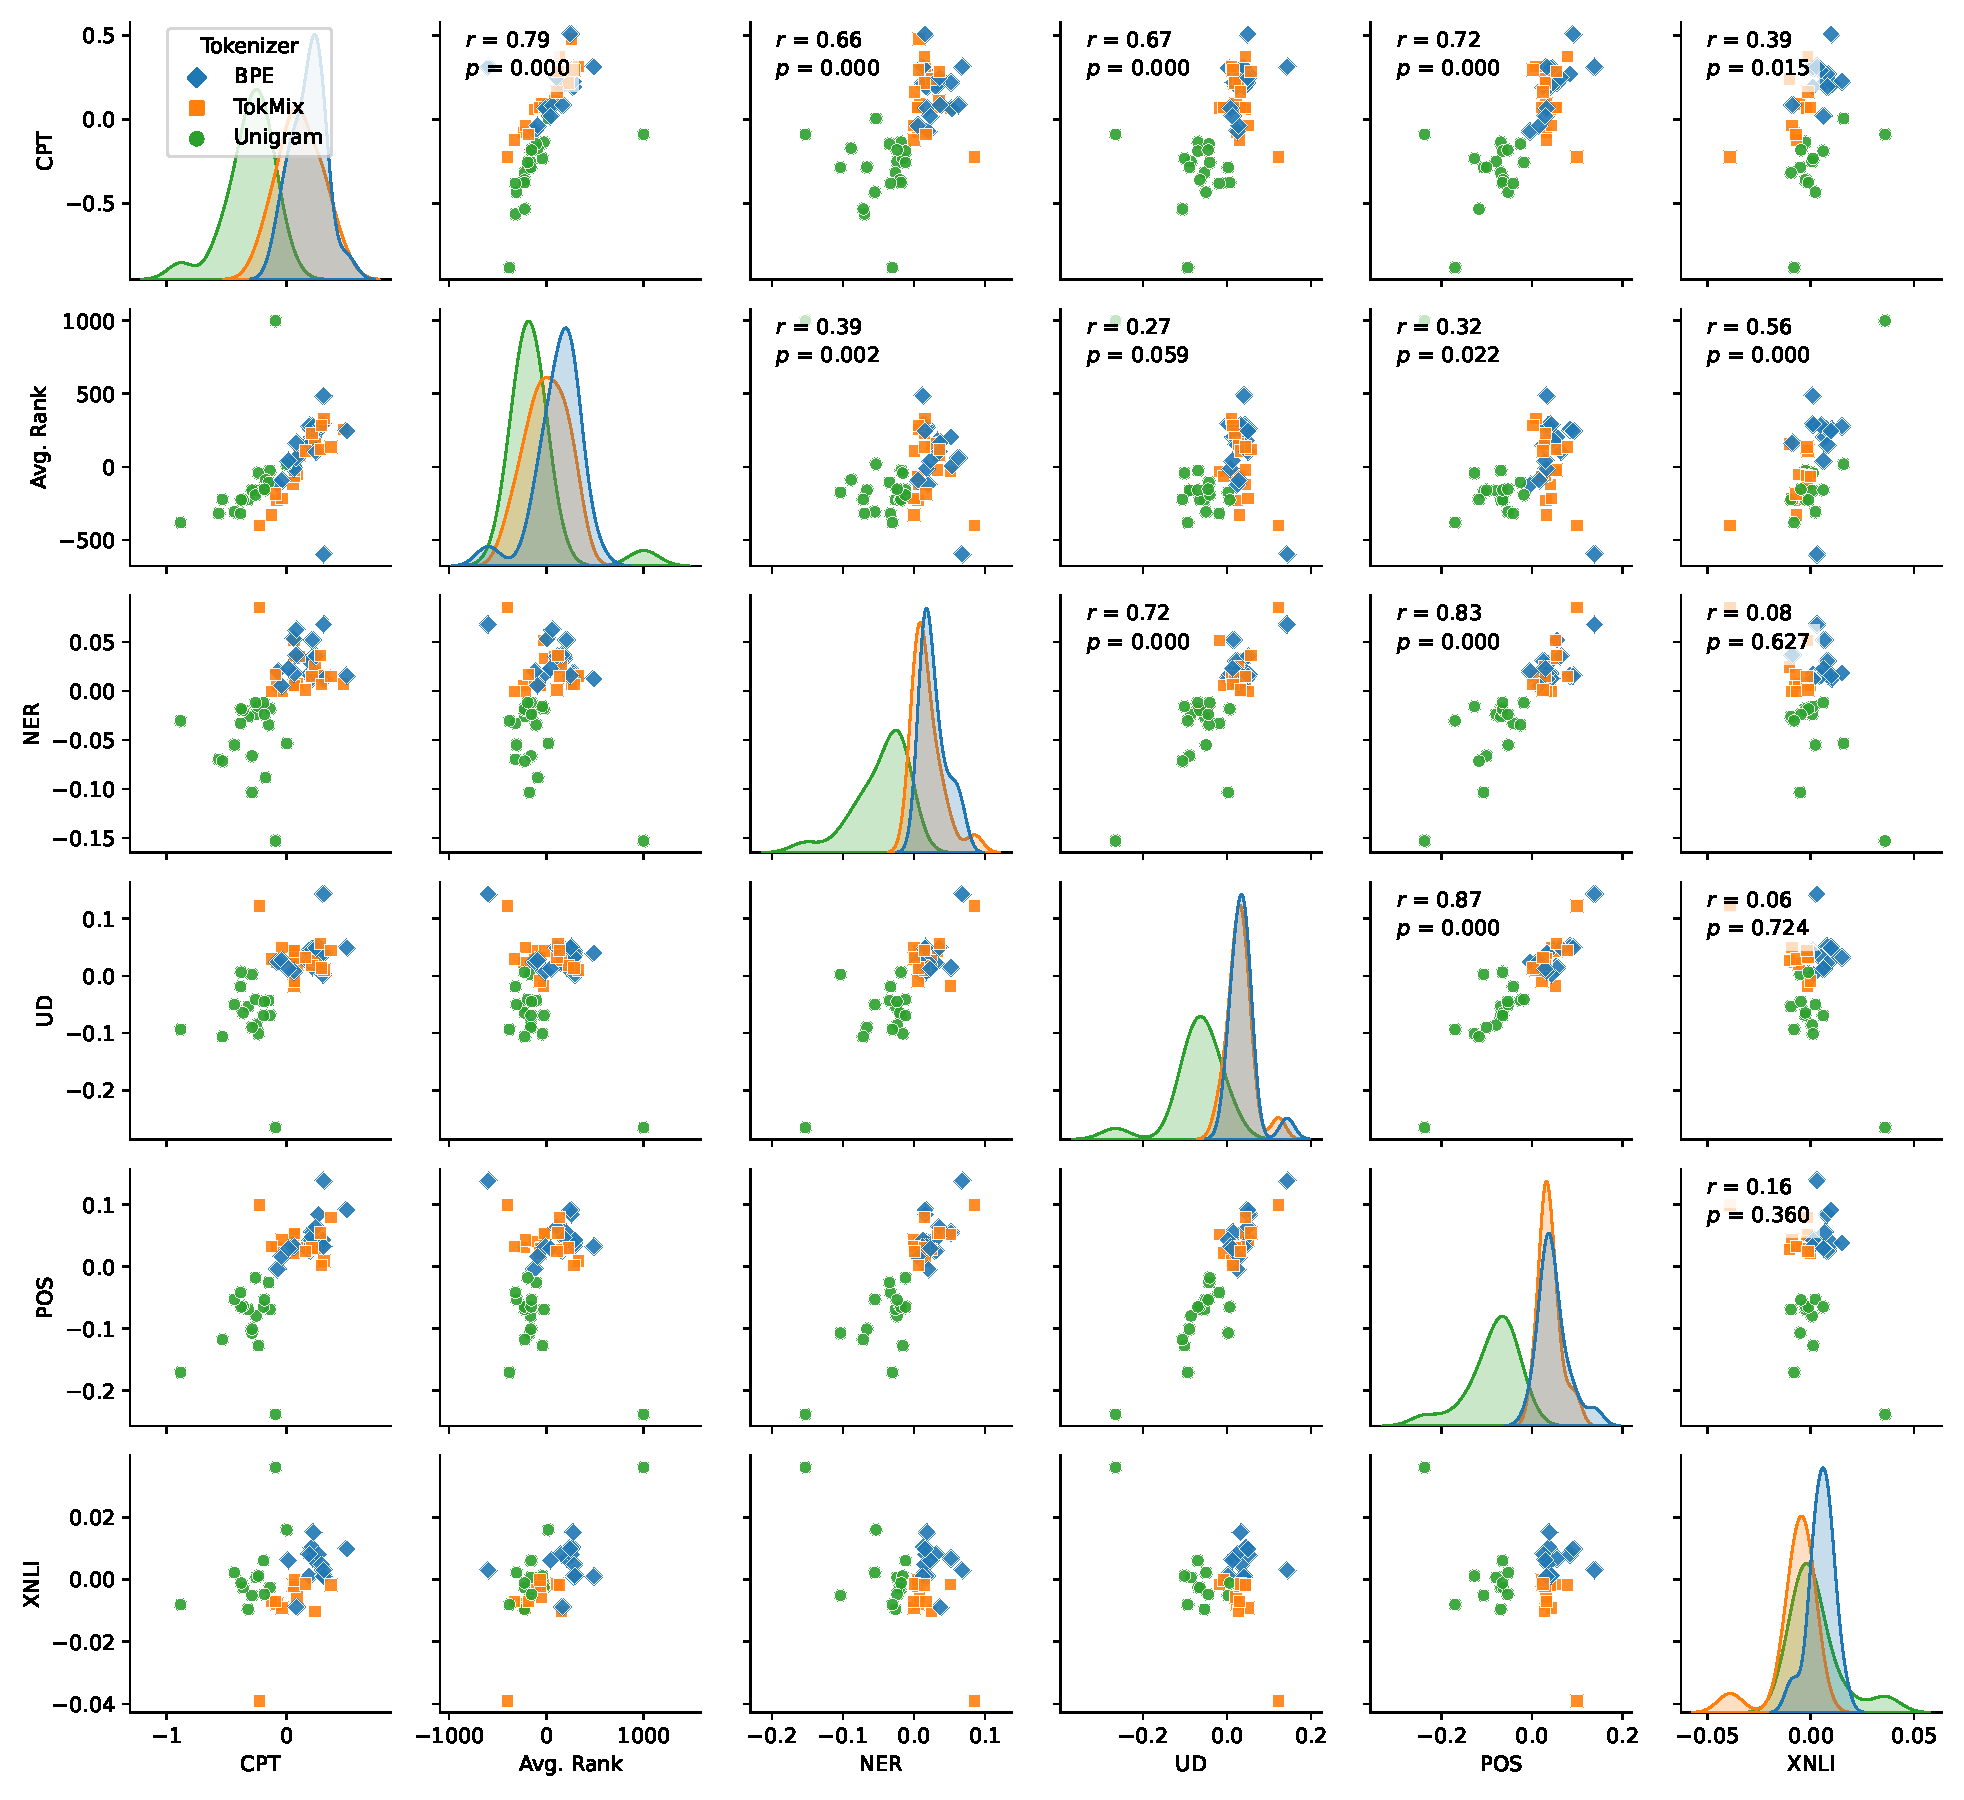
\includegraphics[width=\textwidth]{figures/pair_analysis_20L.pdf}
    \caption{We compare the tokenizer metrics against the contextualized representation quality. For each tokenizer, we pretrain a masked language model, freeze it, and train a linear probe for each task and each of the available languages. We observe a high Spearman correlation between CPT and the word-level tasks (NER, POS, UD) and a high correlation between AR and the sentence-level task XNLI. This suggests that our vocabulary allocation metrics are good indicators of the tokenizer's quality and higher vocabulary allocation leads to better downstream performance. Each data point corresponds to an average result over three seeds of probe training and evaluating one of the languages. The results for each language are centered around the mean to account for the differences between languages.}
    \label{fig:pair_analysis_20L}
\end{figure}

\begin{figure}[H]
    \centering
    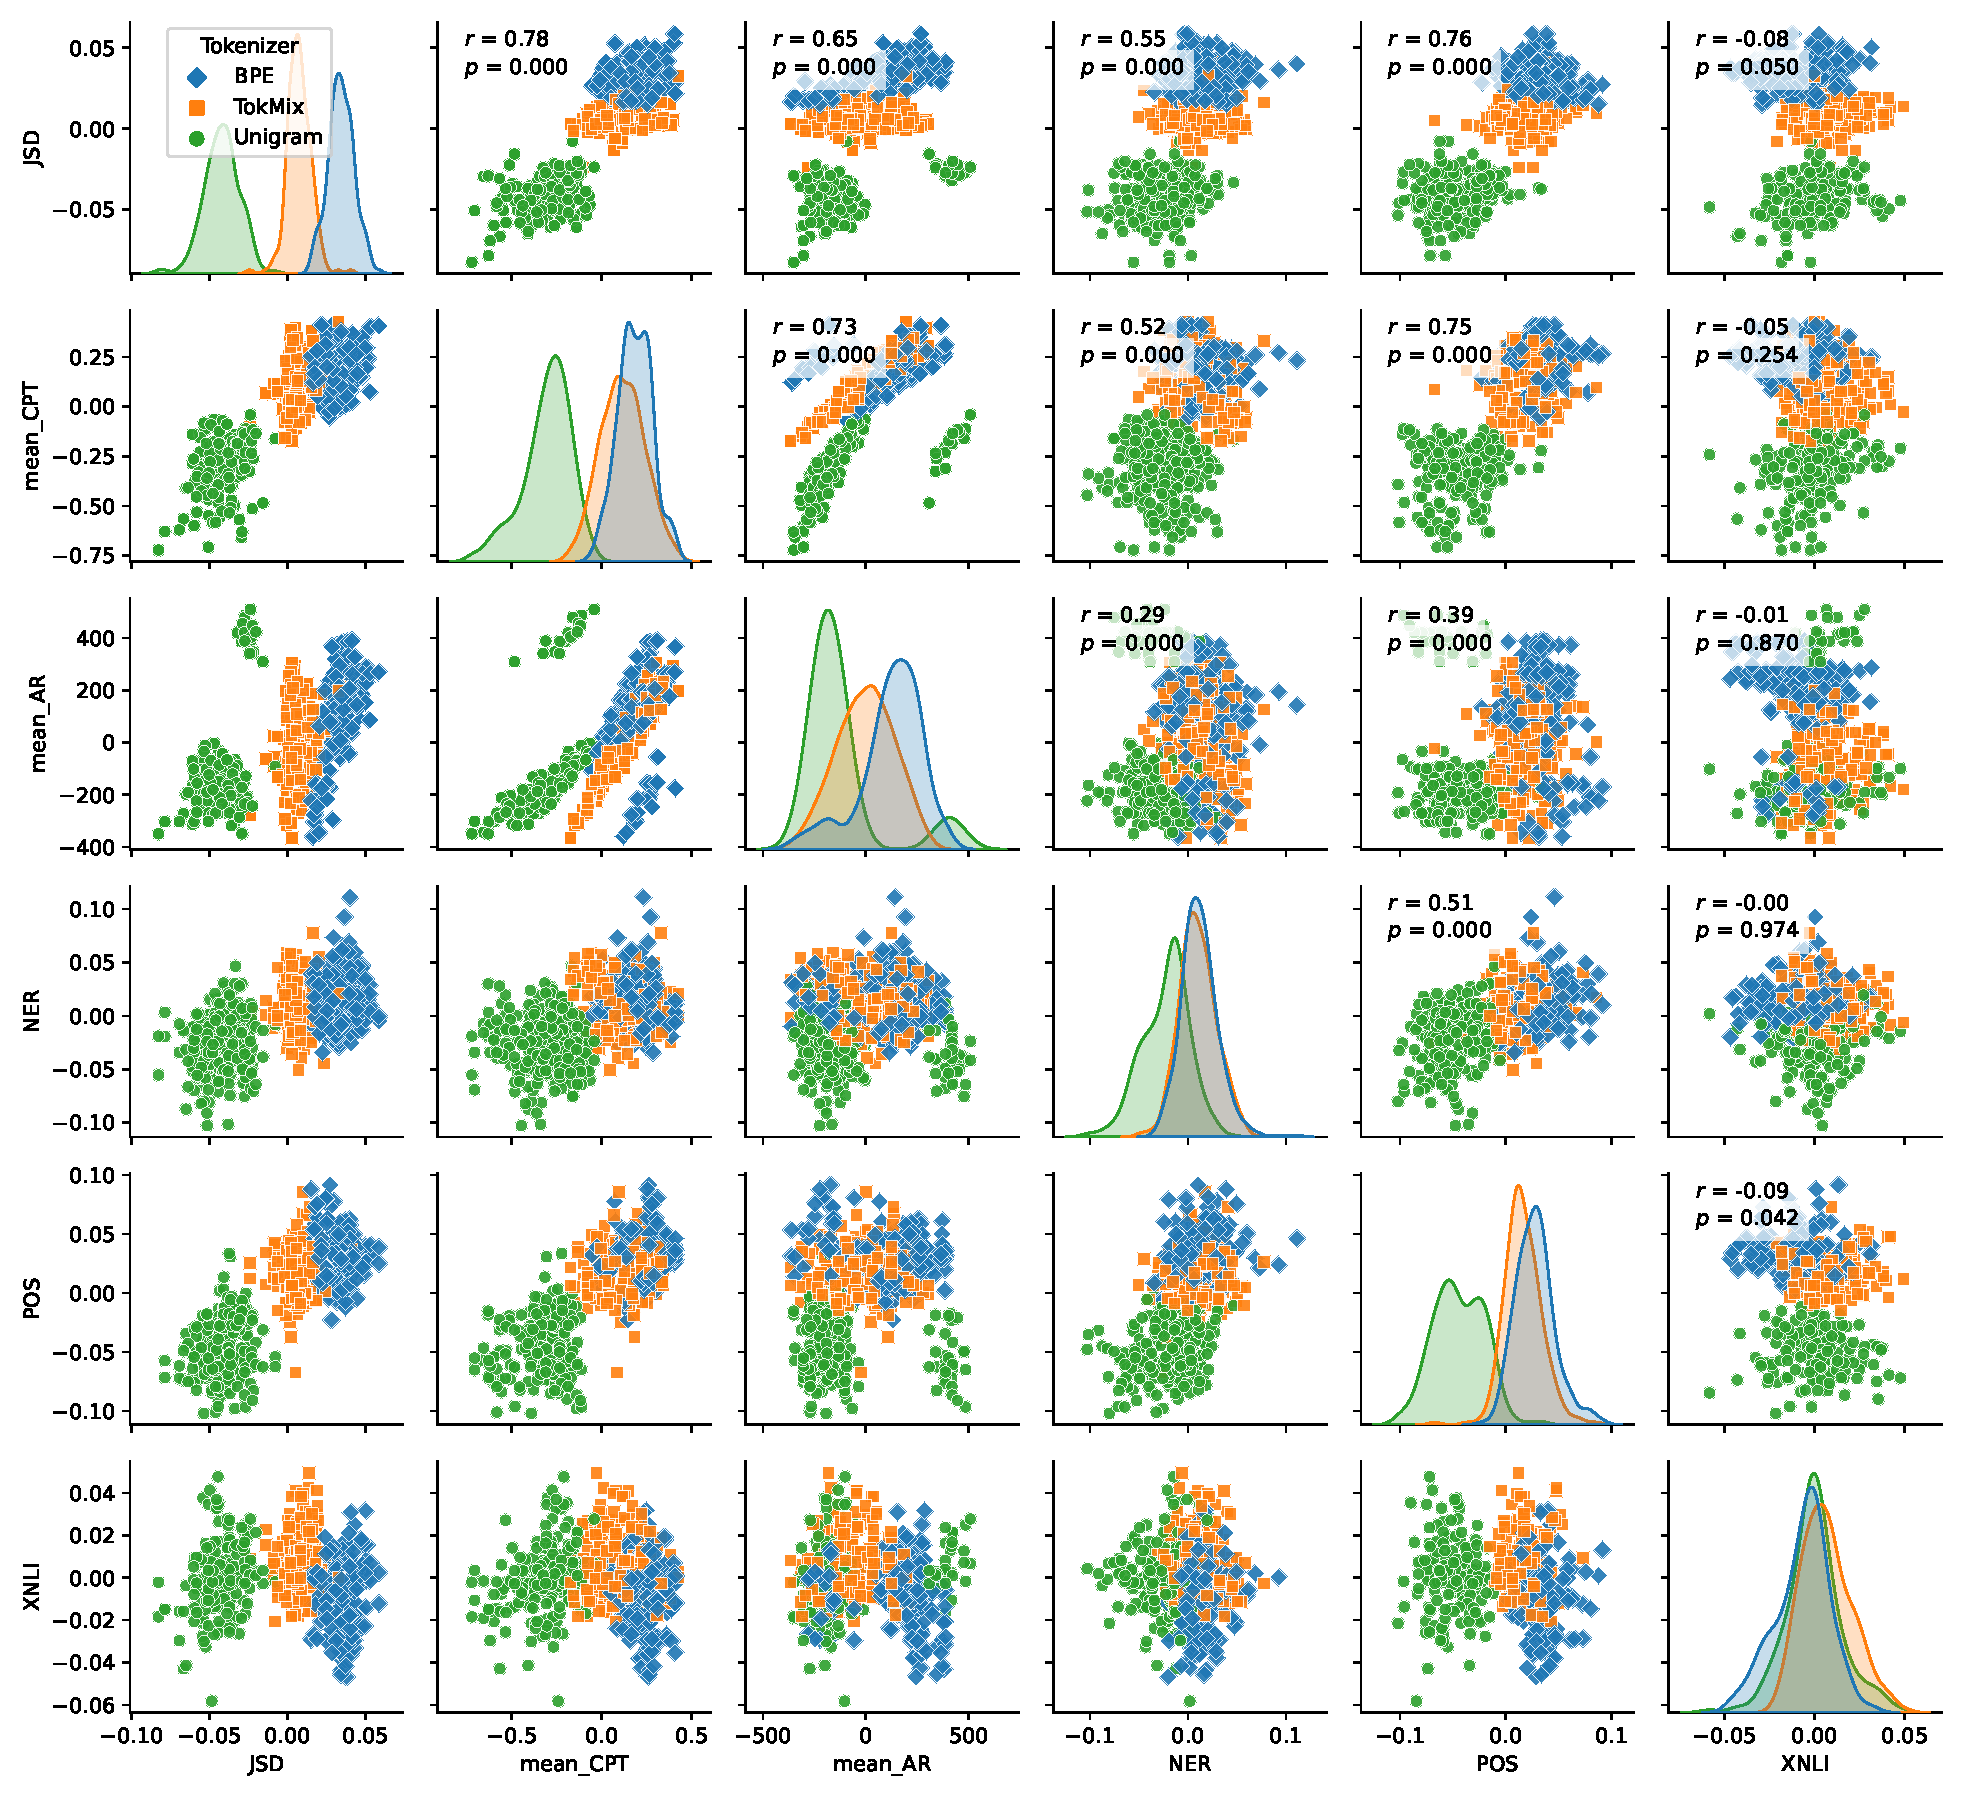
\includegraphics[width=\textwidth]{figures/X_pair_analysis_20L.pdf}
    \caption{We compare the tokenizer metrics against the cross-lingual performance of the models. For each tokenizer, we pretrain a masked language model, freeze it, and train a linear probe on each of the available languages. Then we evaluate the models on all languages the probe has \textbf{not} been trained on, assessing the cross-lingual properties of the model. Here we observe a high correlation between JSD and the word-level tasks, especially the POS and UD. This suggests that less overlap (higher divergence) between the vocabularies of the languages leads to better cross-lingual performance for word-level tasks.
    \xxx{remove the ar and cpt metrics?}} 
    \label{fig:X_pair_analysis_20L}
\end{figure}

\begin{table}
\centering

\begin{tabular}{lcc}
\toprule
 & \multicolumn{2}{c}{\bf{V. Allocation}} \\
 & (AR) &  (CPT) \\
\midrule
CPT    &    \bf{0.790} &     - \\
NER    &   \bf{0.394} &   \bf{0.657}  \\
POS    &     0.320 &   \bf{0.724} \\
Dep l. &     0.266 &   \bf{0.675} \\
NLI   &    \bf{0.56} &    0.388 \\ 
\bottomrule
\end{tabular}
\caption{Spearman correlations between centered in-language task results and tokenizer measures. Statistically significant correlations ($p<0.01$) are bolded.}
\label{tab:corr_in_lang_20l}
\end{table}
\begin{table*}
\centering
\begin{tabular}{lcccccc}
\toprule
 & \bf{V. Overlap} & \multicolumn{2}{c}{\bf{V. Allocation SRC}}  & \multicolumn{2}{c}{\bf{V. Allocation TGT}} \\ 
 & (JSD) &  (AR)  &  (CPT) & (AR) & (CPT) \\ \midrule
% NER     &  \bf{-0.153} &        0.061 &  \bf{0.174} &   \bf{0.180} &   \bf{0.250} \\
% POS     &   \bf{0.164} &       \bf{0.187} &  \bf{0.366} &       \bf{0.238} &  \bf{0.379} \\
% Dep l.     &   \bf{0.095} &      \bf{ 0.095} &  \bf{0.216} &       \bf{0.134} &  \bf{0.232} \\
% NLI    &  \bf{-0.234} &         -0.060 &   -0.025 &       -0.079 &   -0.071 \\
% Retrieval &  \bf{-0.157} &         0.041 &    0.023 &         0.031 &     0.020 \\
NER     &  \bf{0.553} &       \bf{0.172} &  \bf{0.412} &      \bf{0.409} &  \bf{0.568} \\
POS     &  \bf{0.759} &       \bf{0.383} &   \bf{0.69} &       \bf{0.436} &  \bf{0.714} \\
Dep l.     &  \bf{0.596} &       \bf{0.314} &  \bf{0.587} &       \bf{0.351} &  \bf{0.605} \\
NLI    &  -0.078 &        -0.039 &   -0.006 &       -0.083 &  -0.082 \\
Retrieval &  \bf{0.156} &       \bf{0.214} &  \bf{0.139} &       \bf{0.214} &  \bf{0.144} \\
\bottomrule
\end{tabular}
\caption{Spearman correlations between cross-lingual transfer results and tokenization measures. vocabulary overlap~is measured by JSD, we also measure the correlation with vocabulary allocation s of source and target language of the transfer directions. Statistically significant correlations ($p<0.01$) are bolded. Computed for 20 languages.}
\label{tab:corr_x_lang_20l}
\end{table*}


% \begin{figure}[H]
%     \centering
%     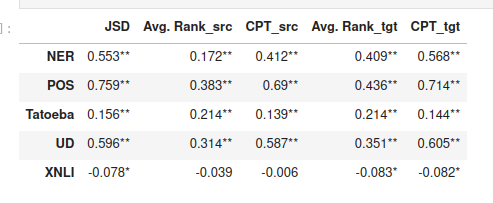
\includegraphics[width=\textwidth]{img/temp/corr_x_lang_20l.png}
%     \caption{Correlations between task cross-lingual transfer results and tokenization measures."Stars denote statistical significance: (* coresponeds to $p<0.05$ and ** to $p<0.01$).\xxx{remove the ar and cpt metrics? Merge with the previous correlation table?}}
%     \label{fig:corr_x_lang_20l}
% \end{figure}

% ---------

\section{The choices that influence the tokenizers quality}
\tomasz{Desceibe potential sources of differences between tokenizers in experiment part. Here just write the results.}

\subsection{Implementation}
\label{sec:implementation}

\begin{table}
\caption{In this table, we compare the Huggingface and Sentencepiece implementations of the Unigram and BPE algorithms. As shown, the Huggingface Unigram tokenizer is a clear outlier in terms of all metrics. We can see that this is a problem in the implementation as the corresponding Sentencepiece \textit{unigram\_alpha0.3} scores much higher. As we will explore in \ref{tab:coverage_influence}, the different alphabet size does not influence the metrics enough to explain the difference. \xxx{here I can add an experiment with the same alphabet size, to be able to skip the reference} Interestingly, we found that the BPE implementation (\textit{huggingface\_bpe\_alpha0.25}) is better in Huggingface than in Sentencepiece (\textit{bpe\_alpha0.25}).}
\label{tab:hugg_vs_sentpiece}
\begin{tabular}{lrrrrr}
\toprule
Tokenizer & Alphabet & \# UNKs & CPT & AR & JSD \\
\midrule
huggingface\_bpe\_alpha0.25 & 1000 & 14040.1 & 3.713 & 1253.7 & 0.783 \\
unigram\_alpha0.3 & 2666 & 923.5 & 3.702 & 1190.7 & 0.768 \\
bpe\_alpha0.25 & 1215 & 7235.6 & 3.666 & 1212.9 & 0.774 \\
huggingface\_unigram\_alpha0.25 & 12616 & 4.5 & 3.204 & 1010.5 & 0.745 \\
\bottomrule
\end{tabular}
\end{table}


As shown in the previous \autoref{sec:influence_of_metrics}, we observe that the Huggingface Unigram tokenizer leads to significantly worse metrics than the other tokenizers. We investigate this difference by turning to the original Sentencepiece implementation of the algorithm and running a comparable experiment. For comparison, we also train a comparable BPE tokenizer using the Sentencepiece library. All tokenizers are trained with vocabulary size 120\,000.

The results are presented in \autoref{tab:hugg_vs_sentpiece}. We see that the implementation has an effect on tokenization. We compare the Sentencepiece Unigram tokenizer (\textit{unigram\_alpha0.25\_alphabet}) trained on the same data and with the same parameters as the Huggingface Unigram (\textit{huggingface\_unigram\_alpha0.25}). We see that there is a large difference between the two. Huggingface Unigram underperforms all of our tokenizers. On the other hand, the Sentencepiece Unigram approaches the metrics of the BPE tokenizers. We further see that if we restrict the vocabulary size for the Sentencepiece Unigram (\textit{unigram\_alpha0.3}), we close the gap between Unigram and BPE. 

Interestingly, we observe that the Huggingface implementation of BPE (\textit{huggingface\_bpe\_alpha0.25}) seems to be better than the Sentencepiece implementation of BPE (\textit{bpe alpha0.25}) in our experimental setup, yielding higher vocabulary allocation metrics (CPT and AR).

Because of the subpar implementation of the Unigram algorithm in the Huggingface library, we use the Sentencepiece implementation for the rest of the experiments.

\subsection{Data size}
\label{sec:data_size}

\begin{table}
\centering
\caption{We measure how much data is generally needed for the tokenizer training. We train handful of Sentencepiece Unigram tokenizers on different amounts of balanced multilingual data. We observe that after 100k-1M lines per language, the tokenizers converge to similar vocabulary allocation and overlap scores. The significance of this experiment is that we find out experimentally how much data is needed for the tokenizer training and we can use this information to make sure that we provide enough data for each language for the further experiments.}
\label{tab:data_size_influence}
\begin{tabular}{rrrrrr}
\toprule
 Lines per language &  Alphabet size &  Number of UNKs &      CPT &          AR &      JSD \\
\midrule
               1000 &           3598 &          520.35 & 3.301636 &  958.414048 & 0.765687 \\
              10000 &           4725 &          117.75 & 3.597563 & 1089.112498 & 0.765236 \\
             100000 &           5041 &           65.55 & 3.695797 & 1192.201089 & 0.767133 \\
            1000000 &           5079 &           62.60 & 3.702038 & 1204.659073 & 0.767357 \\
            1500000 &           5176 &           55.90 & 3.705119 & 1210.664835 & 0.767348 \\
            2000000 &           5180 &           56.35 & 3.705109 & 1212.489940 & 0.767327 \\
\bottomrule
\end{tabular}
\end{table}


We are interested in how much data is needed for the tokenizer training. For this experiment, we sample the same number of lines ($1\times10^{3}, 1\times10^{4}, 1\times10^{5}, 1\times10^{6}, 1.5\times10^{6} \text{ and } 2\times10^{6} \text{ per language}$) for each language from the CC100 corpus. Then we train Sentencepiece Unigram tokenizers on different amounts of data and compare the results in \autoref{tab:data_size_influence}. We see that the metrics improve with the amount of data, but the improvement is not substantial after 100k-1M lines per language. We use these results as a rule of thumb for the rest of the experiments and where possible, we use at least 100k but preferrably 1M lines per language.

\subsection{Character coverage}
\label{sec:character_coverage}

\begin{table}
\caption{We check the tradeoff of including a large alphabet size. We train Sentencepiece Unigram tokenizers with a different target character coverage and observe the resulting alphabet size, number of UNKs and tokenizer metrics. We observe that the alphabet size grows with the coverage and the number of UNKs decreases, as expected. We observe that at both extremes of the character coverage parameter, the vocabulary allocation decreases. The results indicate that the alphabet size between 1000 and 5000 provides a good tradeoff between the number of UNKs and the allocation metrics, while including all characters in the alphabet does not come with a significant decrease in the allocation metrics (-0.05 CPT).}
\label{tab:coverage_influence}
\begin{tabular}{lrrrrr}
\toprule
Coverage & Alphabet & \# UNKs & CPT & AR & JSD \\
\midrule
98.0\% & 539 & 17386.5 & 3.631 & 1115.3 & 0.749 \\
99.5\% & 1136 & 7786.9 & 3.702 & 1173.1 & 0.765 \\
99.95\% & 2678 & 910.6 & 3.705 & 1196.7 & 0.768 \\
99.995\% & 4813 & 83.0 & 3.695 & 1188.7 & 0.769 \\
99.9995\% & 8226 & 10.2 & 3.678 & 1164.2 & 0.769 \\
100.0\% & 13658 & 1.9 & 3.650 & 1124.1 & 0.768 \\
\bottomrule
\end{tabular}
\end{table}


% Because we  observe a large difference in the alphabet size between Huggingface tokenizers (implied by the use of the default trainer settings of the library), we investigate the influence of this parameter on our tokenizer metrics. 
We are also interested in the influence of the alphabet size on our metrics. The alphabet of a tokenizer is the set of characters that are included in the vocabulary. 
We train the Sentencepiece Unigram tokenizers with different character coverage (98\%, 99.5\%, 99.95\%, 99.995\%, 99.9995\%, and 100.0\%) on data sampled with $\alpha=0.3$ from CC100. We show the results in \autoref{tab:coverage_influence}. The character coverage parameter determines, how many distinct Unicode characters are included in the vocabulary of the tokenizer. As expected, we see that there is a direct relationship between the character coverage, alphabet size, and the number of unknown tokens in the validation set. We also see that our metrics are not largely affected by the alphabet size, as the alphabet accounts for at most 10\% of the whole vocabulary size 120\,000. The lowest vocabulary allocation metrics are on the extremes of the character coverage parameter, where the resulting alphabet size is either very small or very large. We assume that the small alphabet size leads to a large number of unknown tokens and the tokenizer is forced to segment words containing characters outside of the alphabet, as these unknown tokens might even be characters with diacritics. In the range of 1000-5000 alphabet size, we see that the metrics are not largely affected by the alphabet size. On the other extreme, where alphabet size is large, we suspect that the alphabet starts to take up a larger portion of the vocabulary and the tokenizer has less capacity for longer tokens which we observe as a lower overall CPT and AR. We note that the observed differences are small and including all characters in the training set does not come with a large decrease in our tokenizer metrics (-0.05 CPT and -70 AR compared to 99.95\% coverage). For later experiments, we use the Sentencepiece default character coverage of 99.95\%. When comparing tokenizers with different alphabet sizes, we are aware of the fact that the metrics might be affected by the alphabet size and we take this into account when interpreting the results.

\section{Tokenizer training with data imbalance}
\label{sec:tokenizer_training_with_data_imbalance}

\begin{table}
\caption{We train five Sentencepiece Unigram tokenizers on increasingly imbalanced multilingual dataset. We see that the macro averaged metrics decrease with the increasing imbalance, suggesting that on average, the tokenizer represents the languages less well.}
\label{tab:data_balance_metrics}
\begin{tabular}{lrrrrr}
\toprule
Tokenizer & Alphabet & \# UNKs & CPT & AR & JSD \\
\midrule
Unigram $\alpha$=0.0 & 2975 & 617.1 & 3.712 & 1212.9 & 0.767 \\
Unigram $\alpha$=0.3 & 2666 & 923.5 & 3.702 & 1190.7 & 0.768 \\
Unigram $\alpha$=0.5 & 2859 & 729.0 & 3.618 & 1143.8 & 0.769 \\
Unigram $\alpha$=0.7 & 2733 & 883.2 & 3.556 & 1107.1 & 0.770 \\
Unigram $\alpha$=1.0 & 2476 & 1286.3 & 3.442 & 1041.8 & 0.772 \\
\bottomrule
\end{tabular}
\end{table}


In this section, we present the tokenizers that become the baselines for comparing the related works we replicate. Our experiments with the data imbalance follow the original tokenizer training recipe from XLM-R and mBERT. The method is training the tokenizers on a corpus created by combining monolingual data in different proportions. On one extreme we have the $\alpha=1.0$, where all data available for each language is combined. On the other, we have $\alpha=0.0$, where the data is sampled per line from each language with the same probability. 

The contribution of our method is investigating how the language imbalance affects each language individually using the metrics we have proposed. Moreover, we investigate how the other proposed methods relate to all settings of $\alpha$, not only to the unbalanced settings of $\alpha=0.5 \textrm{ or } 0.7$ as is done in \citet{chung_improving_2020,zheng_allocating_2021,liang_xlm-v_2023}.

\tomasz{Again, don't mix setup with results!}
For the data balancing experiment, we train 5 tokenizers with a vocabulary size of 120\,000 on an increasingly imbalanced corpus with $\alpha = 0.0, 0.3, 0.5, 0.7, 1.0$ using the CC100 with 20 languages. For $\alpha = 0.0, 0.3, 0.5, 0.7$ we make sure to sample at least 100k lines per language as we have found this to be important in \autoref{sec:data_size}. We note that the data imbalance for $\alpha=1.0$ is so large, that we needed to settle for 30k-70k training lines for the five least resourceful languages (ka, ur, te, mr, sw) because of memory constraints. We use the Sentencepiece Unigram tokenizer with the default settings. Specifically, we use the default character coverage of 99.95\%. We evaluate the tokenizers on a balanced validation set sampled from a holdout portion of the CC100 corpus. 

The overall results with metrics macro averaged over the 20 languages are presented in \autoref{tab:data_balance_metrics}. The results demonstrate a clear disparity in the quality of tokenization depending on the data balance. Training on balanced data leads to higher overall metrics than on unbalanced data. The imbalance also affects the alphabet size as it is possible to cover 99.95\% of the characters in the training data with a smaller alphabet because of the overrepresentation of a few high-resource languages.

We explore the reason for the decreasing performance of the tokenizers trained on imbalanced data in \autoref{fig:data_balance_vs_allocation_per_lang}. We plot the differences in vocabulary allocation metrics between the most unbalanced tokenizer $\alpha=1.0$ and the rest of the tokenizers. We sort the languages by the data size available starting with the highest-resource languages and ending with the low-resource. We see that the vocabulary allocation metrics for the high-resource languages (en, vi, ru, fr, es, th) are improving with the data imbalance. On the other hand, the low resource languages (ka, ur, te, mr, sw) are disproporionally more affected by the imbalance and their vocabulary allocation metrics are decreasing significantly. This suggests that the marginal benefit of adding more data to the high-resource languages is lower than the incurred cost on the quality of tokenization for the low-resource languages. We see the result of this tradeoff in the \autoref{tab:data_balance_metrics} as an overall decrease in the average CPT and AR.

\begin{figure}[H]
    \centering
    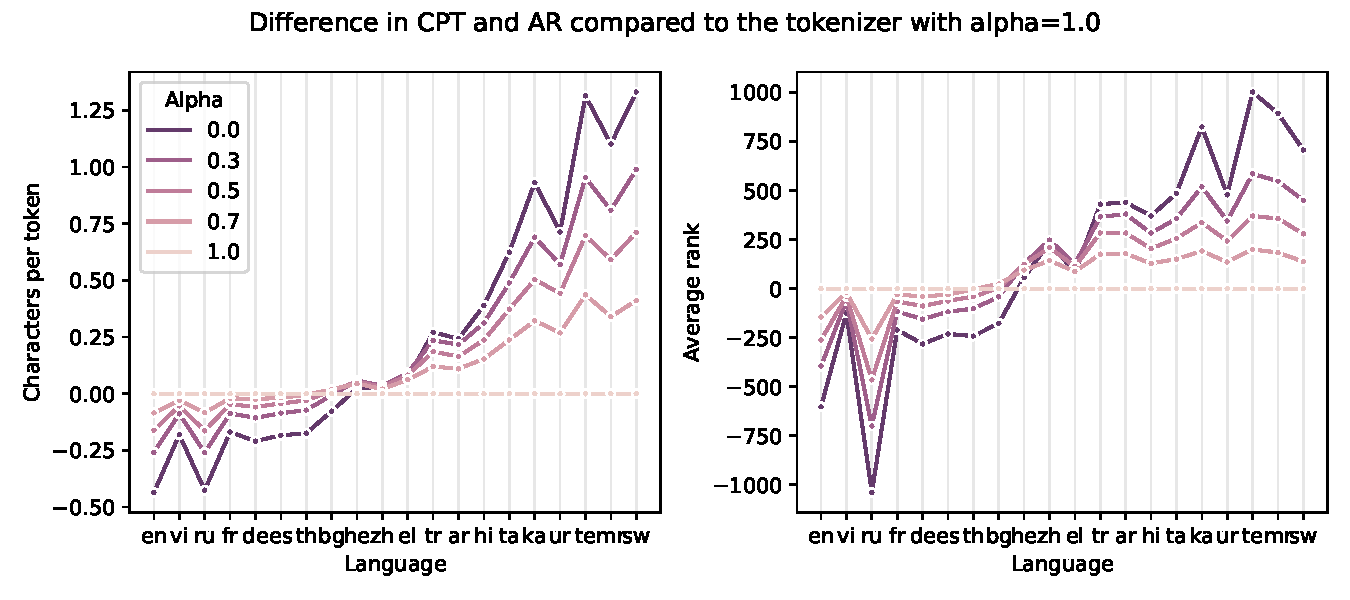
\includegraphics[width=\textwidth]{figures/ar_cpt_vs_alpha.pdf}
    \caption{We examine the impact of the language imbalance on the Sentencepiece Unigram tokenizer training. We train five tokenizers with an increasing language imbalance controlled by the $\alpha$ parameter. Then we look at the effect on the vocabulary allocation metrics per language. We center the results using the most unbalanced tokenizer with $\alpha=1.0$. As expected, the more balanced tokenizers have higher vocabulary allocation scores for low-resource languages and lower scores for high-resource languages. Interestingly, the effect varies across languages. For example, the vocabulary allocation of high-resource Vietnamese or French is not as affected by the decrease in training data as English or Russian.}
    \label{fig:data_balance_vs_allocation_per_lang}
\end{figure}


\section{Comparison of balancing methods}
\label{sec:comparison_balancing_methods}

\begin{table}
\caption{In this summary table, we present all tokenizers used in this chapter. Along with the Huggingface tokenizers from table \ref{fig:20l_metrics} and Sentencepiece Unigram tokenizers from \ref{fig:data_balance_vs_allocation_per_lang}, we include the tokenizers obtained by replicating the papers \citet{chung_improving_2020,zheng_allocating_2021,liang_xlm-v_2023} in our setting. As we can see, the Huggingface Unigram tokenizer is a clear outlier in terms of all metrics even after taking account the higher alphabet size as explored in \ref{tab:coverage_influence}. Further we can see that the proposed balancing methods are improving over the baselines the authors used (\textit{unigram\_alpha0.5} and \textit{unigram\_alpha0.7}). On the other hand we see that using more balanced data for training the Sentencepiece Unigram (\textit{unigram\_alpha0.0}) does lead to similar overall performance as the replicated methods.
The rows are sorted by the CPT score. \xxx{As we can see that except for the Huggingface tokenizers, the alphabet sizes for all tokenizers stay in the stable range of 1000-5000. This corresponds to a comparable number number of UNKs in the holdout data.
}}
\label{tab:all_tokenizers_metrics}
\begin{tabular}{lrrrrr}
\toprule
Tokenizer & Alphabet & \# UNKs & CPT & AR & JSD \\
\midrule
huggingface\_bpe\_alpha0.25 & 1000 & 14040.1 & 3.713 & 1253.7 & 0.783 \\
unigram\_alpha0.0 & 2975 & 617.1 & 3.712 & 1212.9 & 0.767 \\
Chung\_20clusters & 4123 & 270.3 & 3.702 & 1098.7 & 0.766 \\
unigram\_alpha0.3 & 2666 & 923.5 & 3.702 & 1190.7 & 0.768 \\
TokMix\_alpha0.25 & 2497 & 1203.2 & 3.691 & 1163.4 & 0.773 \\
Chung\_16clusters & 3933 & 387.1 & 3.677 & 1102.2 & 0.767 \\
Liang\_20clusters & 3709 & 341.4 & 3.676 & 1103.2 & 0.765 \\
Zheng\_20langs & 4854 & 245.7 & 3.673 & 1094.5 & 0.765 \\
Liang\_16clusters & 3655 & 416.8 & 3.669 & 1106.2 & 0.767 \\
bpe\_alpha0.25 & 1215 & 7235.6 & 3.666 & 1212.9 & 0.774 \\
unigram\_alpha0.5 & 2859 & 729.0 & 3.618 & 1143.8 & 0.769 \\
Chung\_8clusters & 4870 & 684.4 & 3.575 & 1061.1 & 0.770 \\
unigram\_alpha0.7 & 2733 & 883.2 & 3.556 & 1107.1 & 0.770 \\
Chung\_4clusters & 3253 & 648.6 & 3.546 & 1071.9 & 0.768 \\
Liang\_8clusters & 4283 & 568.2 & 3.544 & 1081.6 & 0.767 \\
Liang\_4clusters & 3698 & 419.2 & 3.512 & 1082.5 & 0.769 \\
unigram\_alpha1.0 & 2476 & 1286.3 & 3.442 & 1041.8 & 0.772 \\
huggingface\_unigram\_alpha0.25 & 12616 & 4.5 & 3.204 & 1010.5 & 0.745 \\
\bottomrule
\end{tabular}
\end{table}


In this section, we compare the tokenizers we replicated following the works of \citet{chung_improving_2020,zheng_allocating_2021,liang_xlm-v_2023}. For each of the clustering methods (Chung, Liang), we create 4 variants with different numbers of clusters (4, 8, 16, 20) as that is the main hyperparameter of the methods. For Zheng, we create one variant by greedily maximizing the ALP metric across the 20 languages. We present the results alongside the rest of the experiments in this chapter to provide context and be better able to interpret the differences between the methods.

In \autoref{tab:all_tokenizers_metrics}, we compare overall metrics for all tokenizer experiments\footnote{Note that for Sentencepiece Unigram with $\alpha=0.0\text{ and }0.3$ we retrain the tokenizers on 20M and 10M lines of data respectively (compared to 2M and 5M from \autoref{tab:data_balance_metrics}) to match the data provided to the replicated methods. This does not increase the metrics by a lot as observed in \autoref{sec:data_size}. Nevertheless, we wanted to match the data sizes between the reproduced methods and the Unigram baselines.}. We sort the table by the CPT metric. We see that the unbalanced tokenizers ($\alpha=1.0, 0.7$) are placed at the bottom of the results along with the underperforming Huggingface Unigram implementation. We see that generally, the standard tokenizers trained on a balanced dataset provide the best results on our tokenizer metrics. Next, we see the clustering methods of Chung and Liang with 20 and 16 clusters along with the Zheng method. Only then we see the standard tokenizers trained on less balanced or unbalanced datasets and clustering methods with a lower number of clusters. We visualize our vocabulary allocation metrics on a scatterplot in \autoref{fig:all_tokenizers_AR_vs_CPT} to better observe the differences between the tokenizers and explore the relationship between CPT and AR. Each point on the scatterplot is one tokenizer and its position is determined by the CPT and AR metrics. We connect related experiments with a line and color-code them. Here we can see that the tokenizers with high CPT often have high AR. Nevertheless, we also have tokenizers with low AR and high CPT but never the other way around. Our intuition is that it is not possible to construct a tokenizer with a high number of useful tokens which are all very short. With the context of different tokenization methods, we can see the degree of Huggingface Unigram's underperformance.

\begin{figure}[H]
    \centering
    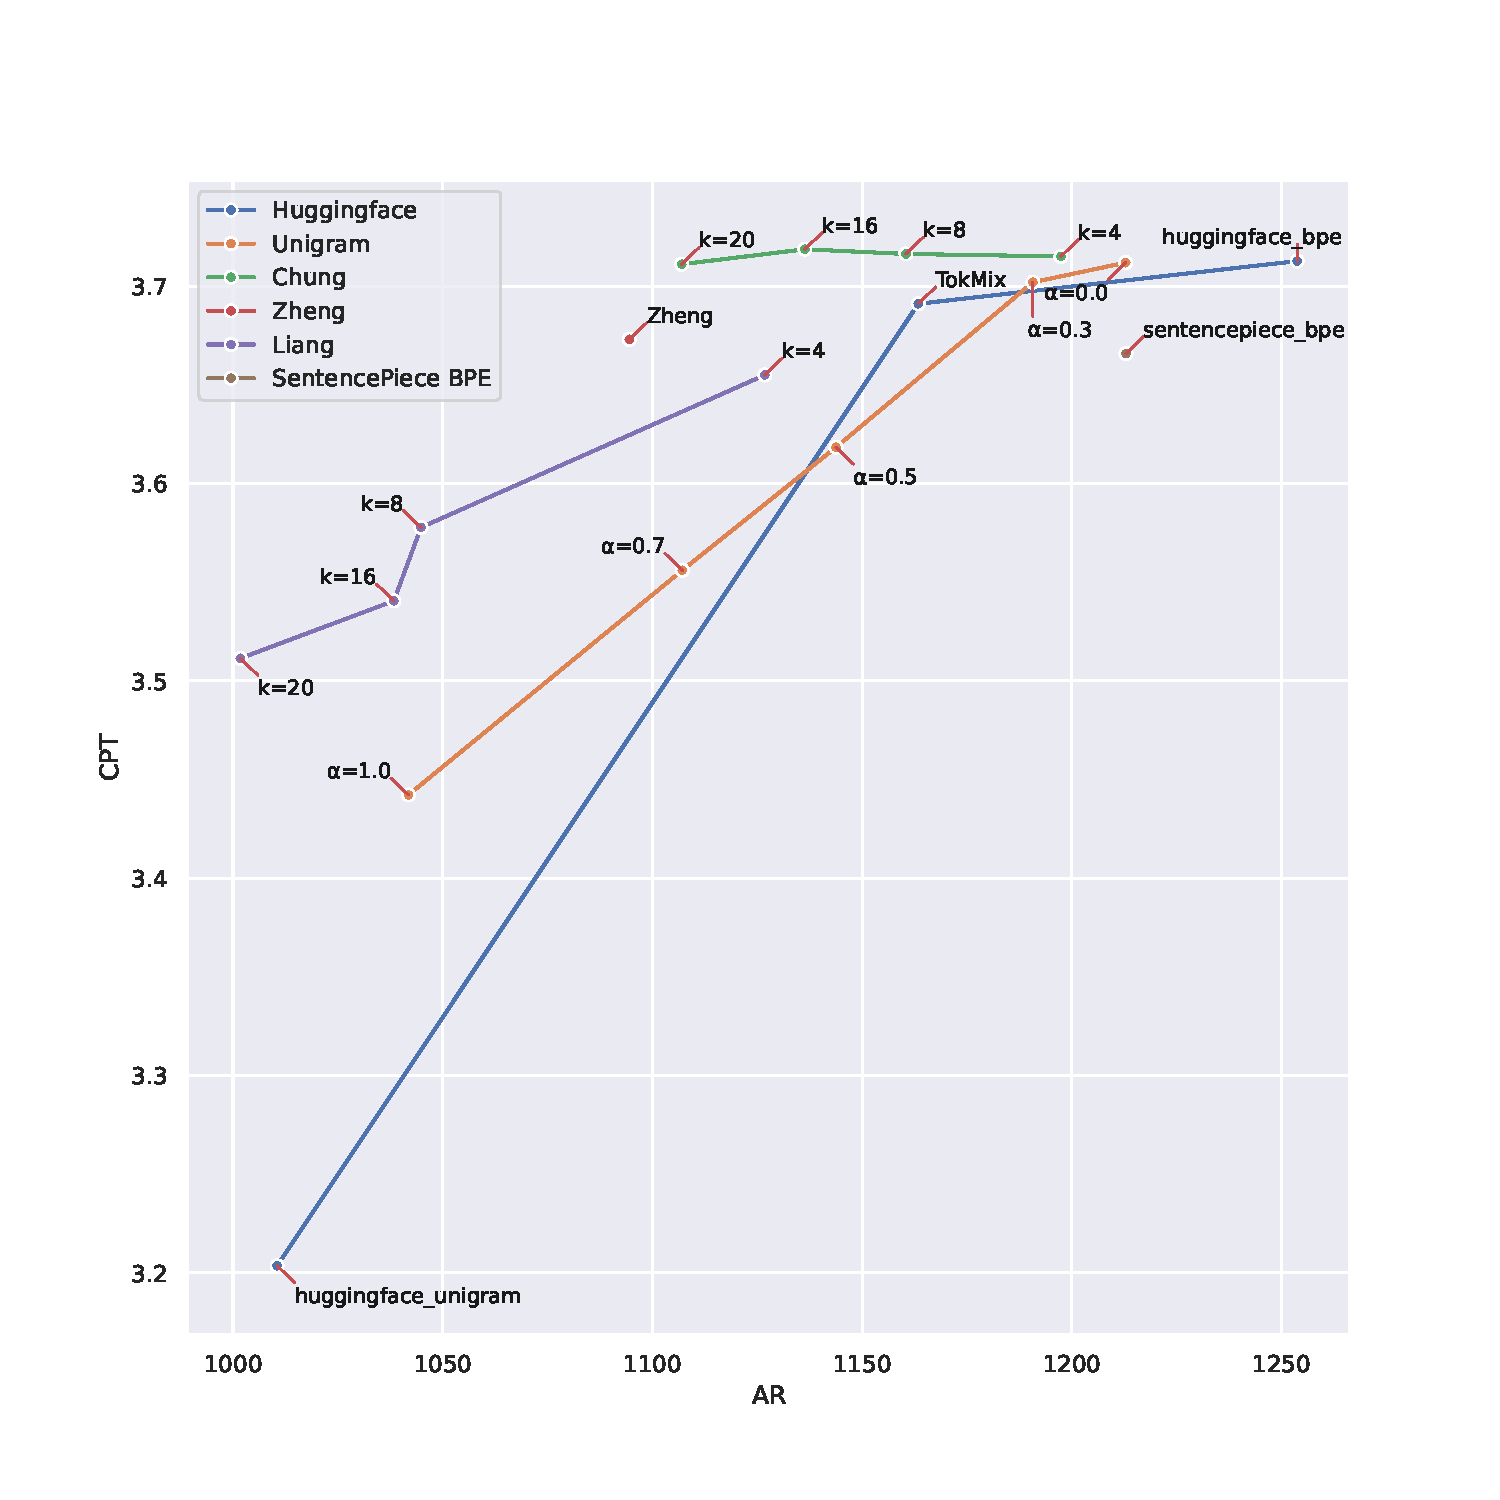
\includegraphics[width=\textwidth]{figures/all_tokenizers_AR_vs_CPT.pdf}
    \caption{We visualize the overall vocabulary allocation metrics for all tokenizers from Table \ref{tab:all_tokenizers_metrics}. We observe that the vocabulary allocation scores are related --- higher AR usually means higher CPT.  We also observe that Huggingface Unigram is a clear outlier, although a combination of separate, monolingual Huggingface Unigrams (TokMix) approaches the performance of the Sentencepiece Unigram with the corresponding data imbalance ($\alpha=0.3$). We see that the balancing methods overperform the unbalanced Unigrams ($\alpha=1.0$, $\alpha=0.7$) in terms of CPT but perform similarly or worse to the simple case of running the Sentencepiece Unigram trainer on a balanced set $\alpha=0.0$.}
    \label{fig:all_tokenizers_AR_vs_CPT}
\end{figure}

Crucially, we see that the reproduced methods of \citet{chung_improving_2020,zheng_allocating_2021,liang_xlm-v_2023} do improve over the unbalanced baselines $\alpha=1.0, 0.7, 0.5$ on the CPT metric, especially with a higher number of clusters but do not outperform the simple case of training the Sentencepiece Unigram on a balanced dataset $\alpha=0.0$. We also observe that the clustering methods with a higher number of clusters along with Zheng are close to each other on the CPT-AR plot. We assume this is because, with higher $k$, the clustering methods reduce to the Zheng method (training separate tokenizers for each language). Similarly, with a lower number of clusters, the methods are much closer to the vanilla Sentencepiece Unigram trained on an unbalanced dataset.

\begin{figure}
    \centering
    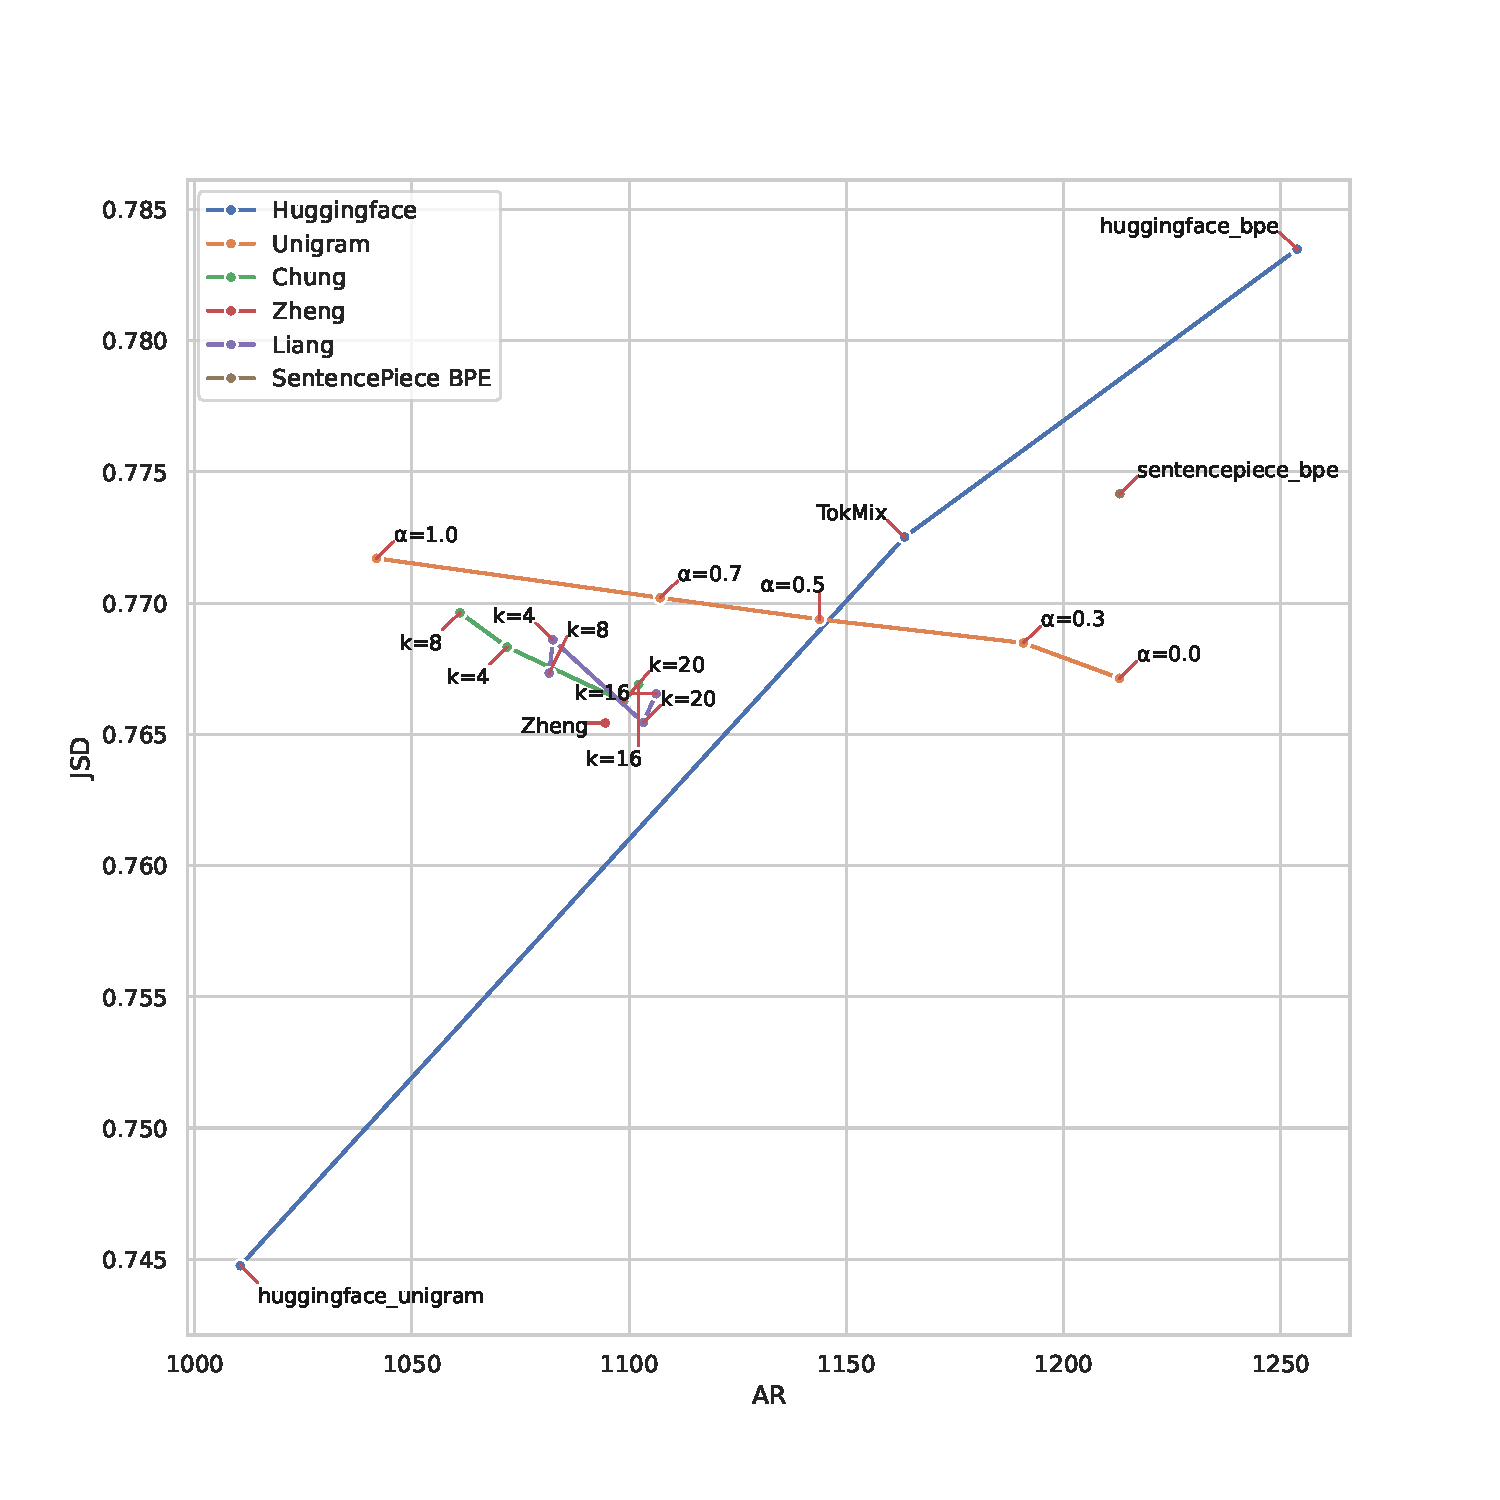
\includegraphics[width=\textwidth]{figures/all_tokenizers_AR_vs_JSD.pdf}
    \caption{We visualize the tokenizers from Table \ref{tab:all_tokenizers_metrics} in terms of Average Rank and Jensen-Shannon Divergence. Here we can see that all methods based on Sentencepiece result in similar overlap independent of the allocation. This is interesting because the replicated balancing methods (Chung, Zheng, Liang) work by splitting the data and training separate tokenizers. Nevertheless, after merging the separate subtokenizers they all seem to end up with similar vocabulary overlaps. The highest vocabulary isolation is surprisingly achieved by the Huggingface BPE tokenizer, which is contrary to the hypothesis stated by \citet{chung_improving_2020,zheng_allocating_2021} that the tokenizers trained on the concatenation of all data tend to select subwords shared across all languages.}
    \label{fig:all_tokenizers_AR_vs_JSD}
\end{figure}

We also explore the relationship between vocabulary allocation and vocabulary overlap on the \autoref{fig:all_tokenizers_AR_vs_JSD}\footnote{The CPT-JSD plot is similar but is less readable therefore we present the relationship between AR and JSD}. We see that the differences between all methods based on Sentencepiece are small compared to the differences between Huggingface tokenizers. This is surprising because one of the motivations for the method of Chung and Liang is to promote overlap between similar languages while minimizing the overlap between distant languages. We would therefore expect the overall overlap to decrease, as the number of spurious token sharing decreases. Nevertheless, we observe that the resulting overlap is lower or similar to our Sentencepiece Unigram tokenizers. Similarly, the Zheng method works by training separate tokenizers for each language and then combining them into one. We would expect the overlap to be even lower than the original Sentencepiece Unigram but we observe that the overlap is comparable. 
Surprisingly, the lowest vocabulary overlap (highest JSD) is achieved by the Huggingface BPE trained on a combined corpus. 

\begin{figure}
    \centering
    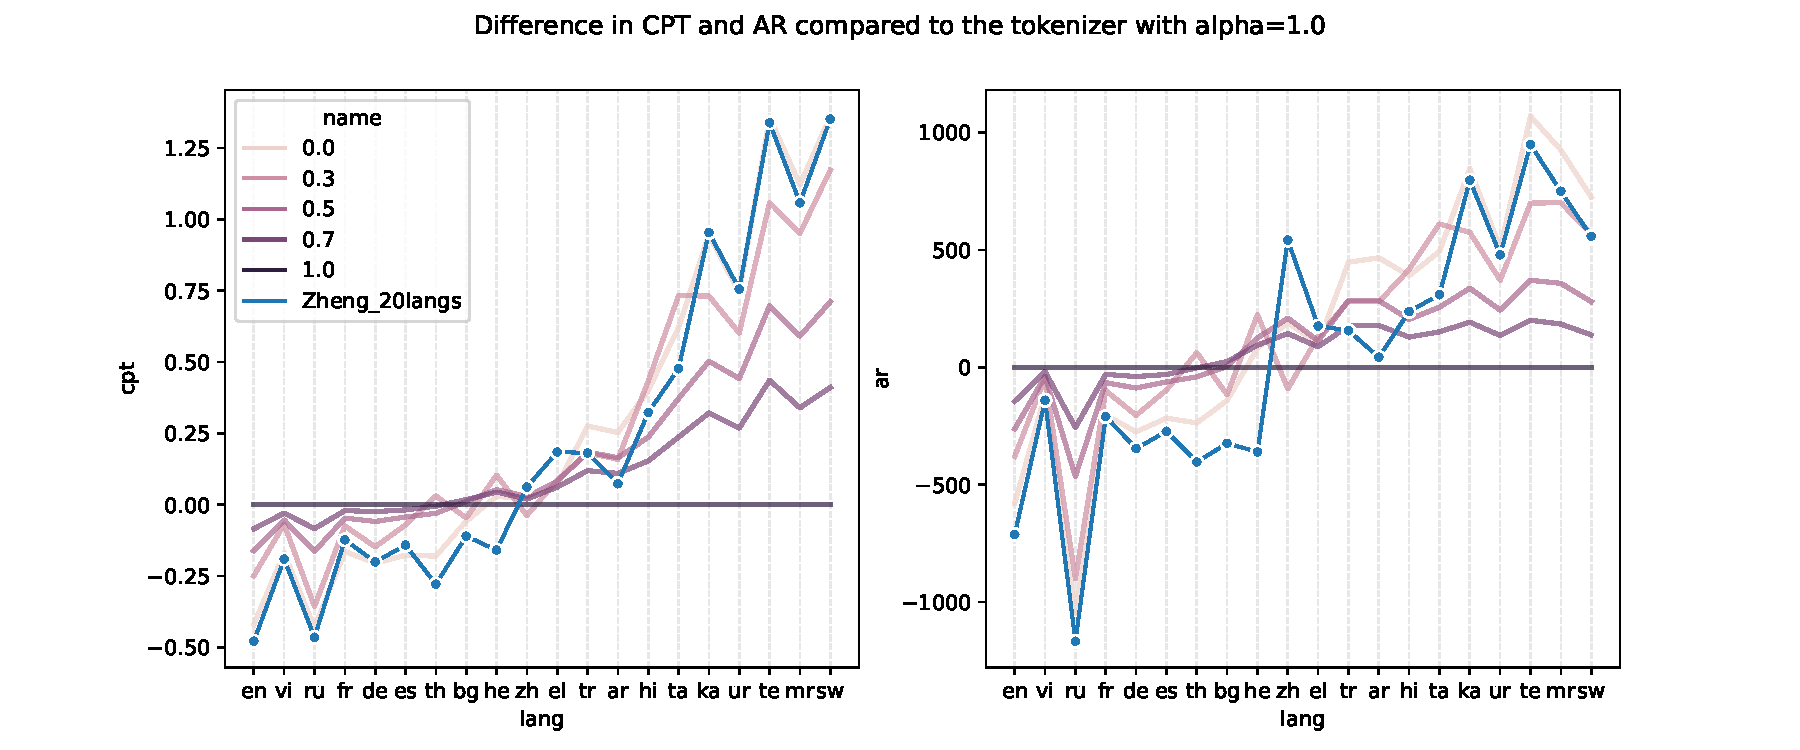
\includegraphics[width=\textwidth]{figures/zheng_vs_alphas.pdf}
    \caption{We zoom into the results of the Zheng method and compare the vocabulary allocation across the individual languages represented by this tokenizer against the backdrop of the vanilla Unigram tokenizers trained with different data imbalances from \ref{fig:data_balance_vs_allocation_per_lang}. We observe a striking similarity between the vocabulary allocation of the Zheng tokenizer and the Unigram tokenizer with $\alpha=0.0$, especially in terms of characters per token. This comes as a large surprise because the Zheng method works by training a separate tokenizer for each language and then merging them. Despite the different methods of obtaining the vocabulary, the resulting tokenizers are very similar across the languages.}
    \label{fig:zheng_vs_alphas}
\end{figure}

We investigate the differences between the balanced Unigram and the replicated methods in more detail by examining the CPT and AR metrics computed \textbf{per language}. We use the data balance experiments from \autoref{sec:tokenizer_training_with_data_imbalance} for comparison. We start by comparing the Zheng method with the increasingly imbalanced Unigram tokenizers in \autoref{fig:zheng_vs_alphas}. We plot the increase or decrease in vocabulary allocation metrics for each language sorted by the data available. Remarkably, we see that the Zheng method is strikingly similar in terms of CPT and AR per language to the Unigram tokenizer trained on the balanced set $\alpha=0.0$. The similarity seems to be higher in the CPT metric although the AR metric is also very similar, especially for the highest and lowest resource languages. We find this result quite surprising because of the distinctness of the Zheng method --- it trains a separate tokenizer for each language and then merges the vocabularies together. Nevertheless, the resulting tokenizers are very similar to the Unigram tokenizer trained on the balanced set. This result seems to validate the choice of the ALP metric for the selection of vocabulary sizes in the Zheng method (see \autoref{fig:zheng_vs_alphas_alp}) but it also calls into question the necessity of the separate training of tokenizers for each language. One advantage of the Zheng method is that splitting the data into separate languages lowers the memory requirements for the training of the separate Sentencepiece Unigram. However, this comes at a cost of higher overall compute time because of the need for training hundreds of tokenizers to be able to select the ones that maximize the overall ALP after merging them.


\begin{figure}[H]
    \centering
    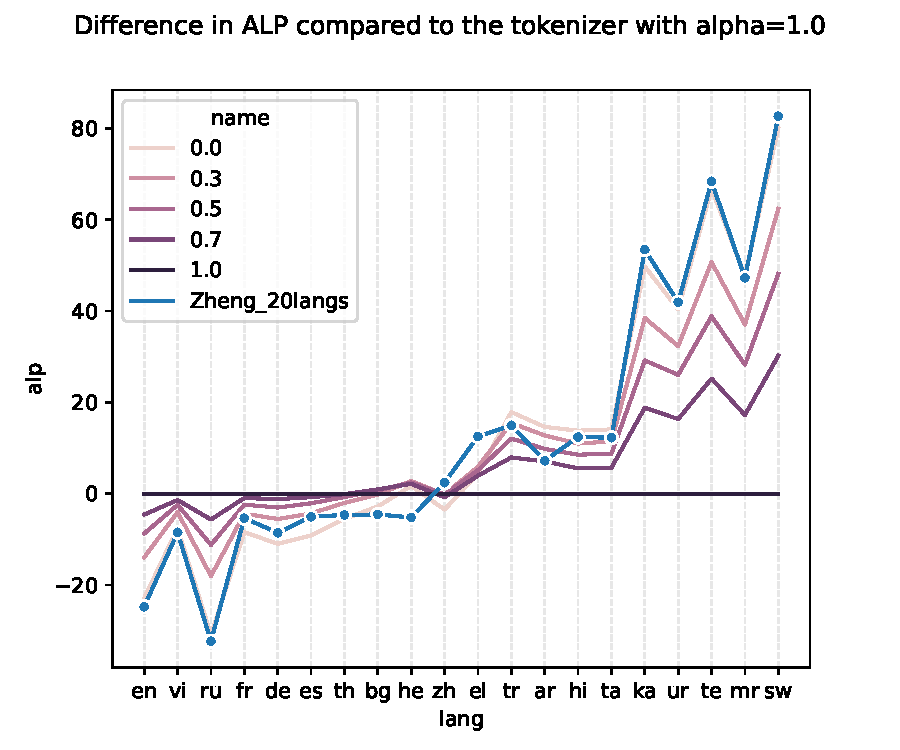
\includegraphics[width=0.7\textwidth]{figures/zheng_vs_alphas_alp.pdf}
    \caption{Intrigued by the similarity between the Zheng tokenizer and the Unigram tokenizer with $\alpha=0.0$ from Figure \ref{fig:zheng_vs_alphas} we also look at the ALP metric which is used for the selection of vocabulary sizes in the Zheng method. Here we see that the greedy optimization of ALP across languages indeed results in a similar vocabulary allocation as the Unigram tokenizer with $\alpha=0.0$.}
    \label{fig:zheng_vs_alphas_alp}
\end{figure}

\begin{figure}[H]
    \centering
    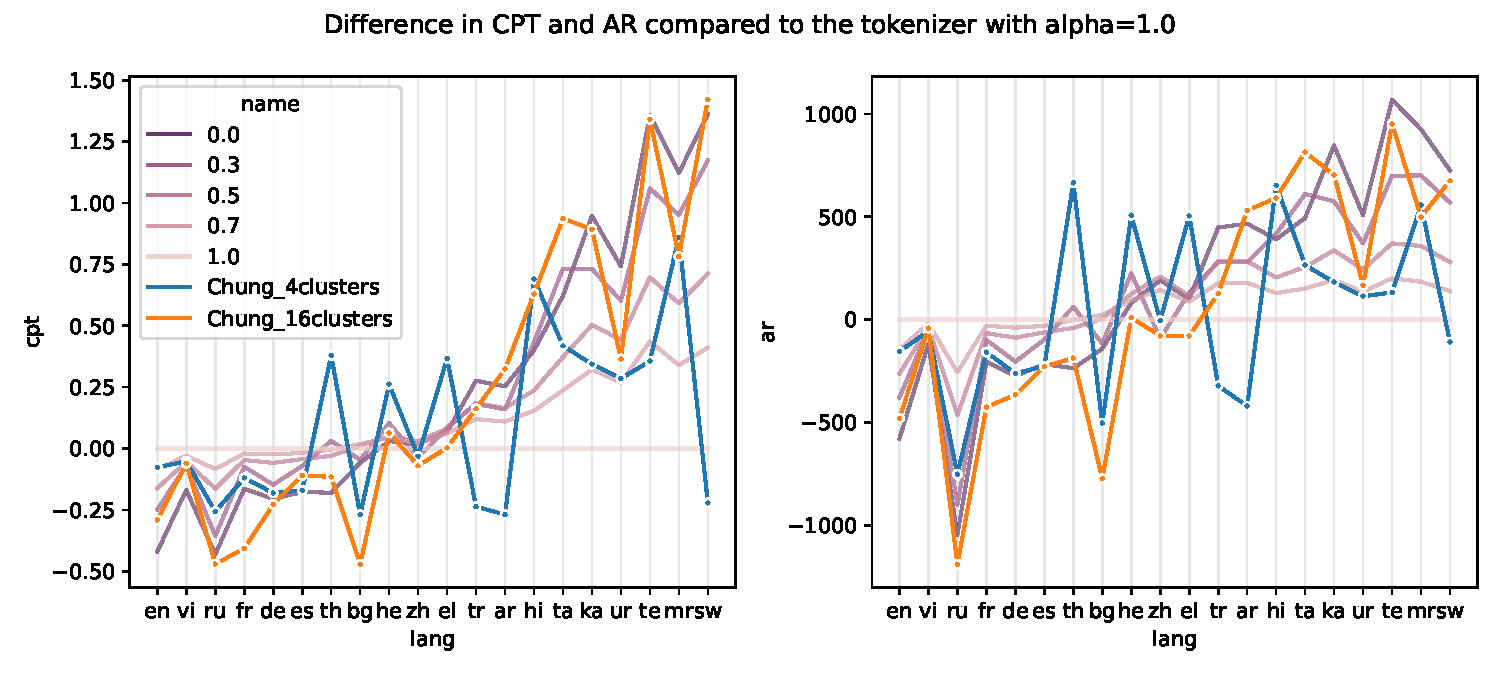
\includegraphics[width=\textwidth]{figures/chung_vs_alphas.pdf}
    \caption{Here we inspect the language-level vocabulary allocation of the Chung method. Similarly to the Zheng method, the Chung method also performs similarly to the Unigram tokenizer with $\alpha=0.0$. Unfortunately, we believe this is an artifact of the choice of our training data for the Chung method. We use a balanced dataset ($\alpha=0.0$) for training the cluster-specific tokenizers. The balance of the data seems to be more important than the clustering step. After merging the cluster-specific tokenizers, the resulting tokenizer is very similar to the Unigram tokenizer with $\alpha=0.0$.}
    \label{fig:chung_vs_alphas}
\end{figure}

Next, we inspect the Chung method and compare it in detail to our Unigram tokenizers in \autoref{fig:chung_vs_alphas}. For comparison, we select a run with a low number of clusters (k=4) and a high number of clusters (k=16). We see that the different numbers of clusters yield different results. In the case of a higher number of clusters, we see that the tokenizer exhibits a similar trend in CPT and AR across the languages as the balanced Unigram tokenizer with $\alpha=0.0$ albeit with some deviations. In the case of a lower number of clusters, the metrics per language seem to be more distinct compared to our Unigram tokenizers. 

We look at the CPT per language for k=16 more closely and identify the languages where the Chung tokenizer differs significantly from the Unigram tokenizer with $\alpha=0.0$. We see that the CPT drops significantly for Bulgarian (bg), Urdu (ur), Marathi (mr), and to some degree French (fr). On the other hand, we see smaller improvements for English (en), Vietnamese (vi), Spanish (es), Thai (th), Hindi (hi), and Tamil (ta). We compare this to the cluster assignments in \autoref{tab:chung_clusters_k16}. Revealingly, we observe that all languages with the large drop in CPT have been assigned to a cluster with another, higher-resource language. Bulgarian is assigned with Russian (8th largest corpus versus 3rd largest corpus), Urdu with Arabic (17th vs. 13th), Marathi with Hindu (18th vs. 14th) and French with English (4th vs. 1st)

We continue with a similar analysis for the 4 clusters. We see that the CPT for Bulgarian (bg), Turkish (tr), Arabic (ar), and Swahili (sw) is lower than any of our Unigram tokenizers. On the other hand, we see significant improvements for Thai (th), Hebrew (he), Greek (el), and Hindi (hi) over our Unigram tokenizers. Additionally, Marathi (mr) achieves the highest CPT increase over the unbalanced Unigram baseline, although the increase stays in the range of the $\alpha=0.5$ Unigram tokenizer. We again look at the cluster assignments in \autoref{tab:chung_clusters_k4}. We observe that Bulgarian and Arabic are assigned to a cluster with higher-resource Russian (3rd) and Chinese, which could explain the decrease in CPT for the two. Similarly, Swahili and Turkish which use the Latin script are assigned to a cluster with higher resource English (largest corpus) and Vietnamese (2nd largest). On the other hand, we see that Thai, Hebrew, and Greek are assigned to a cluster with lower-resource languages --- Tamil (ta), Georgian (ka), Urdu (ur), and Telugu (te). As we have observed, Thai, Hebrew, and Greek benefit from this assignment while the lower-resource languages seem to have a lower CPT than the $\alpha=0.7$ Unigram and therefore approach the unbalanced baseline.

\begin{figure}[H]
    \centering
    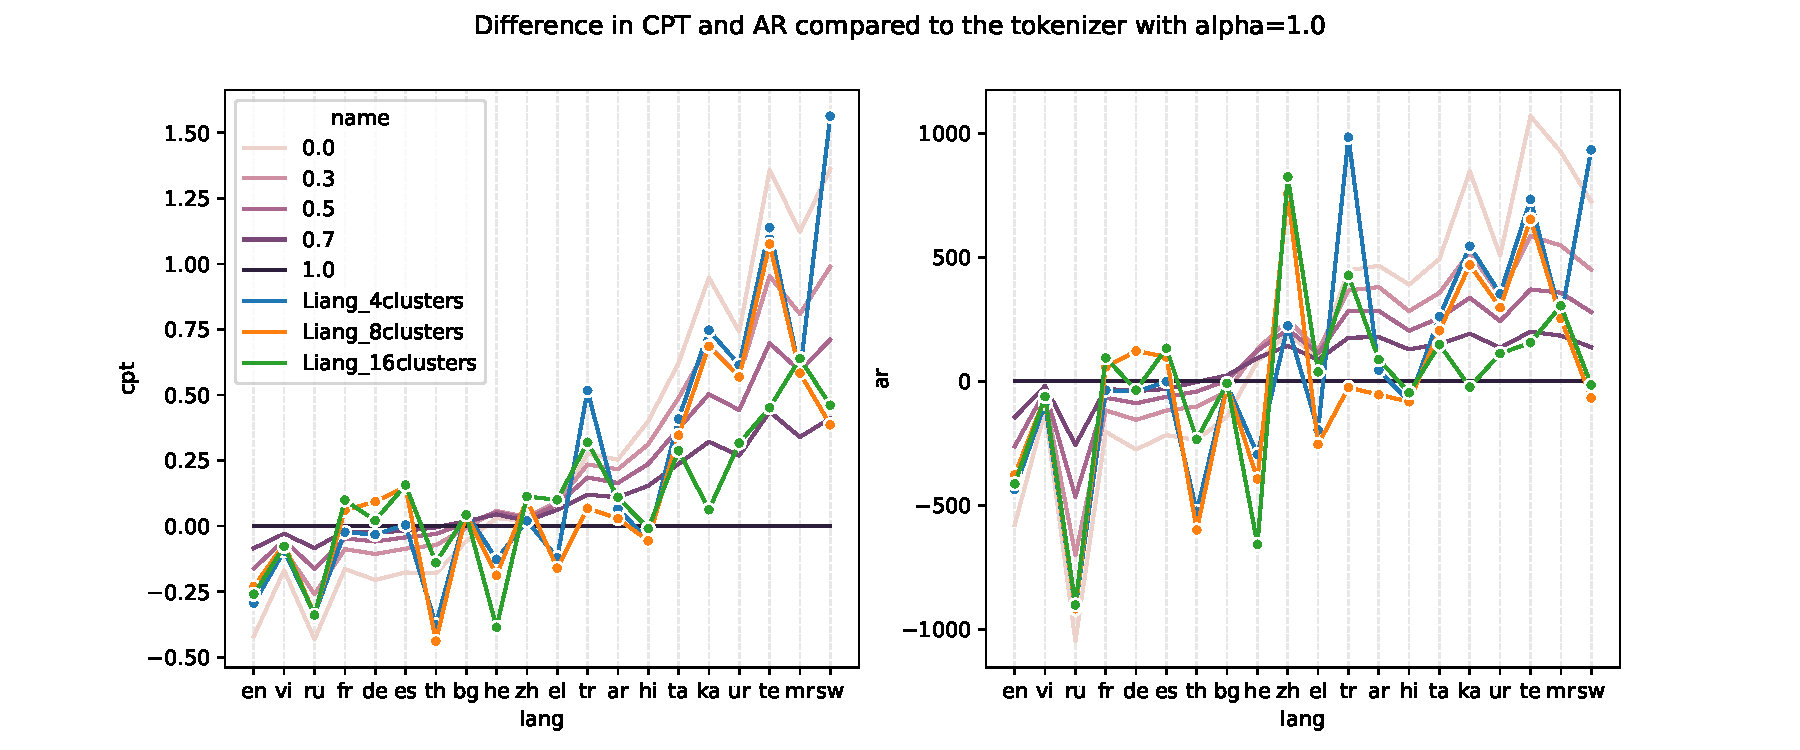
\includegraphics[width=\textwidth]{figures/liang_vs_alphas.pdf}
    \caption{We inspect the language-level vocabulary allocation of the Liang method. We see similarities to the Chung method in \autoref{fig:chung_vs_alphas}. The main differences seem to be the improved Chinese and Arabic for 4 clusters and worse Hebrew and better Urdu for 16 clusters. Overall the results are similar.}
    \label{fig:liang_vs_alphas}
\end{figure}

We look at the \citet{liang_xlm-v_2023} replication results in \autoref{fig:liang_vs_alphas}. We see that despite a slightly different clustering method and per-cluster vocabulary size selection, the Liang method exhibits similar patterns we observed in the Chung method.

Overall, we infer that the Chung and Liang methods are sensitive to cluster assignments. Because the training data are merged per cluster, if a low-resource language gets assigned to a cluster with a high-resource language, the language imbalance acts in favor of the high-resource language. Bearing this in mind, we know from our experiments in \autoref{sec:tokenizer_training_with_data_imbalance} presented previously, that the benefit of adding more data to the high-resource language is lower than the cost that incurs on the low-resource language. We believe this is the cause of the lower overall CPT and AR for the clustering methods.


\section{Comparison of balancing methods on downstream tasks}

To validate our previous assessment from \autoref{sec:comparison_balancing_methods}, we select two replicated methods by \citet{chung_improving_2020,zheng_allocating_2021}. For the clustering method, we select a low- and high- number of clusters $k=4\text{ and }16$. We compare these replicated tokenization methods to the standard Unigram tokenizers trained on differently balanced datasets with $\alpha=1.0, 0.3\text{ and }0.0$

For each of the six tokenizers, we pretrain a masked language model and probe it on three tasks - natural language inference (NLI), part of speech tagging (POS), and named entity recognition (NER). We run the probe training with three different seeds on each language and report the average results\footnote{Note that even though the probe training is done with three different random seeds, the model pretraining was done only once. The variance between pretraining runs is therefore not measured and the error bars should be interpreted as such.}. We note that the models differ only in the tokenizer used. The architecture and training data are fixed across the pretraining and finetuning runs.


\begin{figure}
    \centering
    \begin{subfigure}{.5\textwidth}
      \centering
      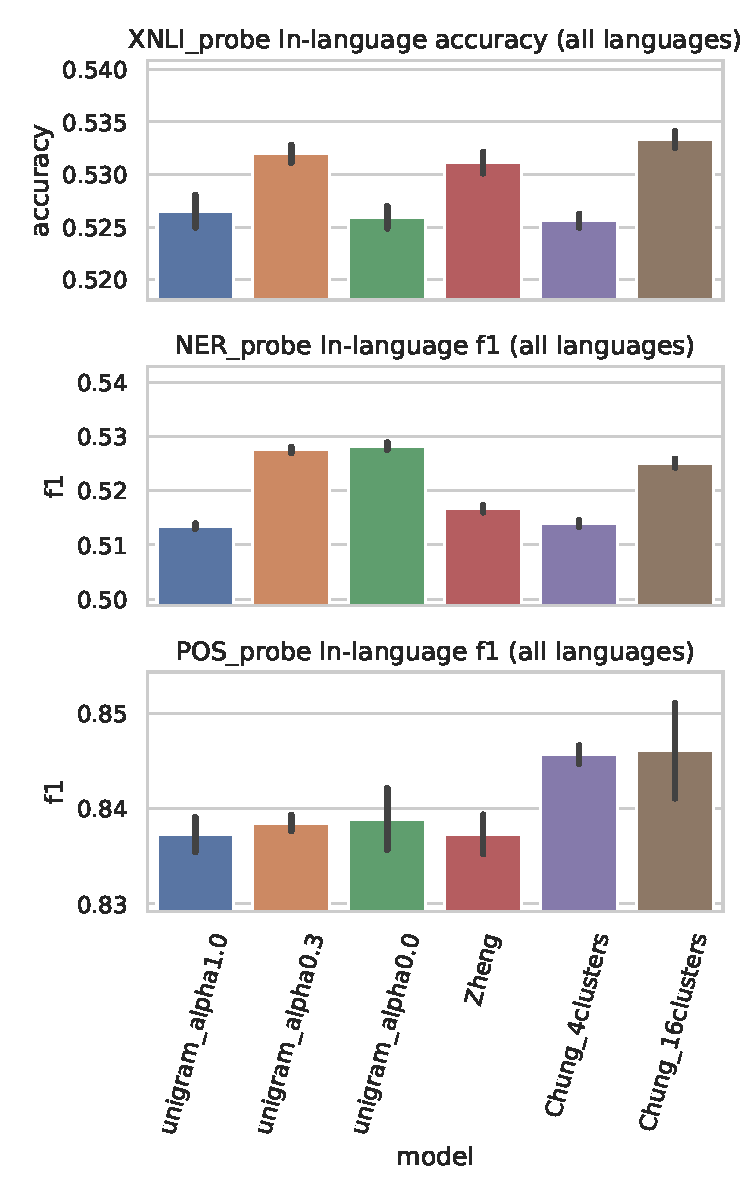
\includegraphics[width=\linewidth]{figures/probe_overall_inlanguage.pdf}
      \caption{In-language results}
      \label{fig:probe_overall_inlanguage}
    \end{subfigure}%
    \begin{subfigure}{.5\textwidth}
      \centering
      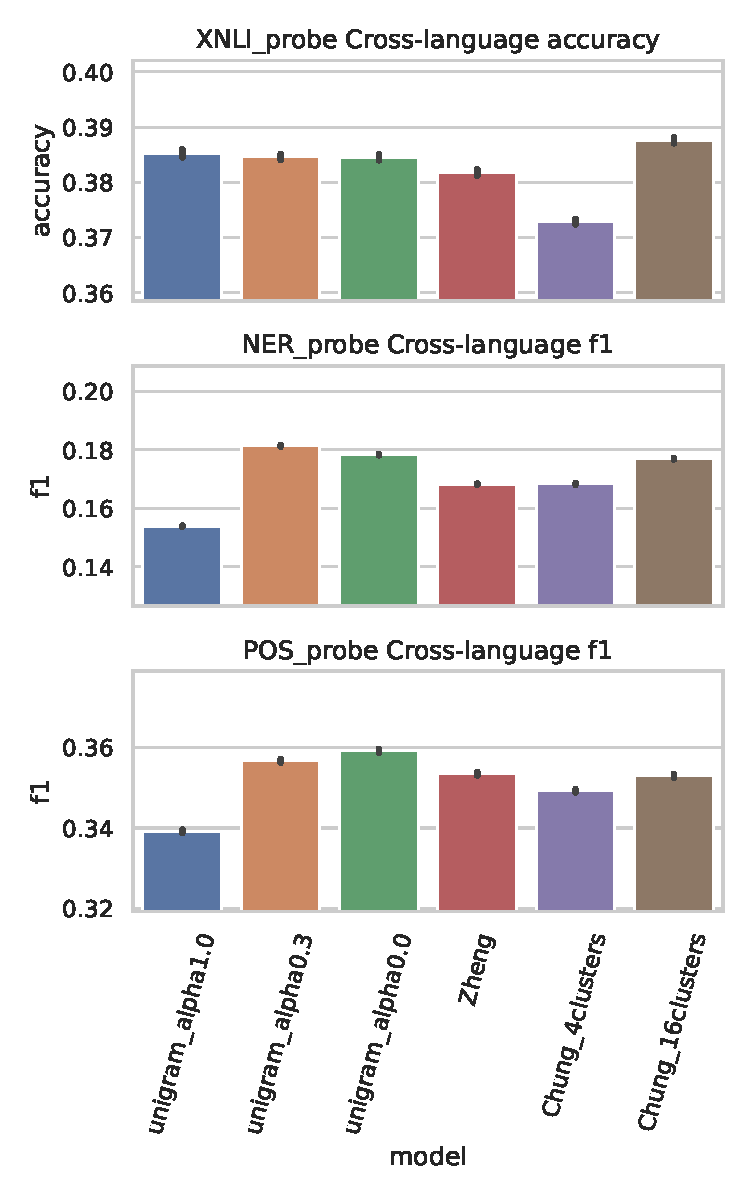
\includegraphics[width=\linewidth]{figures/probe_overall_crosslanguage.pdf}
      \caption{Cross-language results}
      \label{fig:probe_overall_crosslanguage}
    \end{subfigure}
    \caption{We select the replicated methods by \citet{chung_improving_2020,zheng_allocating_2021} and compare them with the vanilla Unigram tokenizers. For comparison, we choose the unbalanced Unigram tokenizer with $\alpha=1.0$ and then two stronger baselines with $\alpha=0.0$ and $\alpha=0.3$ trained on more balanced data. We then pretrain masked language models that differ only in the tokenizer they use and assess the performance of these models on the downstream tasks using probing. We test two settings --- in-language performance, where the model is trained on each of the available languages and then evaluated on the same language, and cross-language performance, where the model is also trained on each language but evaluated on all \textit{but} the training language. The results are a macro average over all the languages (in-language results) or all language pairs (cross-language results). For each model, language, and task we do 3 probe training runs with different random seeds. The error bars represent one standard deviation computed with bootstrapping by randomly sampling seeds for each language.}
    \label{fig:probe_overall}
\end{figure}

In \autoref{fig:probe_overall}, we report the overall in-language and cross-language results for the models. We observe the clearest regularity in cross-language performance for word-level tasks (NER and POS), where all balancing methods improve over the unbalanced $\alpha=1.0$ model. Next, we see higher POS in-language scores for the Chung methods and higher NER in-language scores for the balanced unigrams ($\alpha=0.0\text{ and }0.3$). For in-language NLI, we do not see any systematic effect --- the differences between the models are small ($<1$ percentage point) and the outlier behavior of $\alpha=0.3$ compared to $\alpha=1.0\text{ and }0.0$ suggests that the variance is caused by the finetuning rather than any tokenizer effect.

We inspect the results more closely on the language level. We again compare the performance of the more balanced models to the unbalanced model by plotting the difference in accuracy and F1 score for the tasks by language. The languages are sorted in descending order based on the amount of available data. 



\begin{figure}[H]
    \centering
    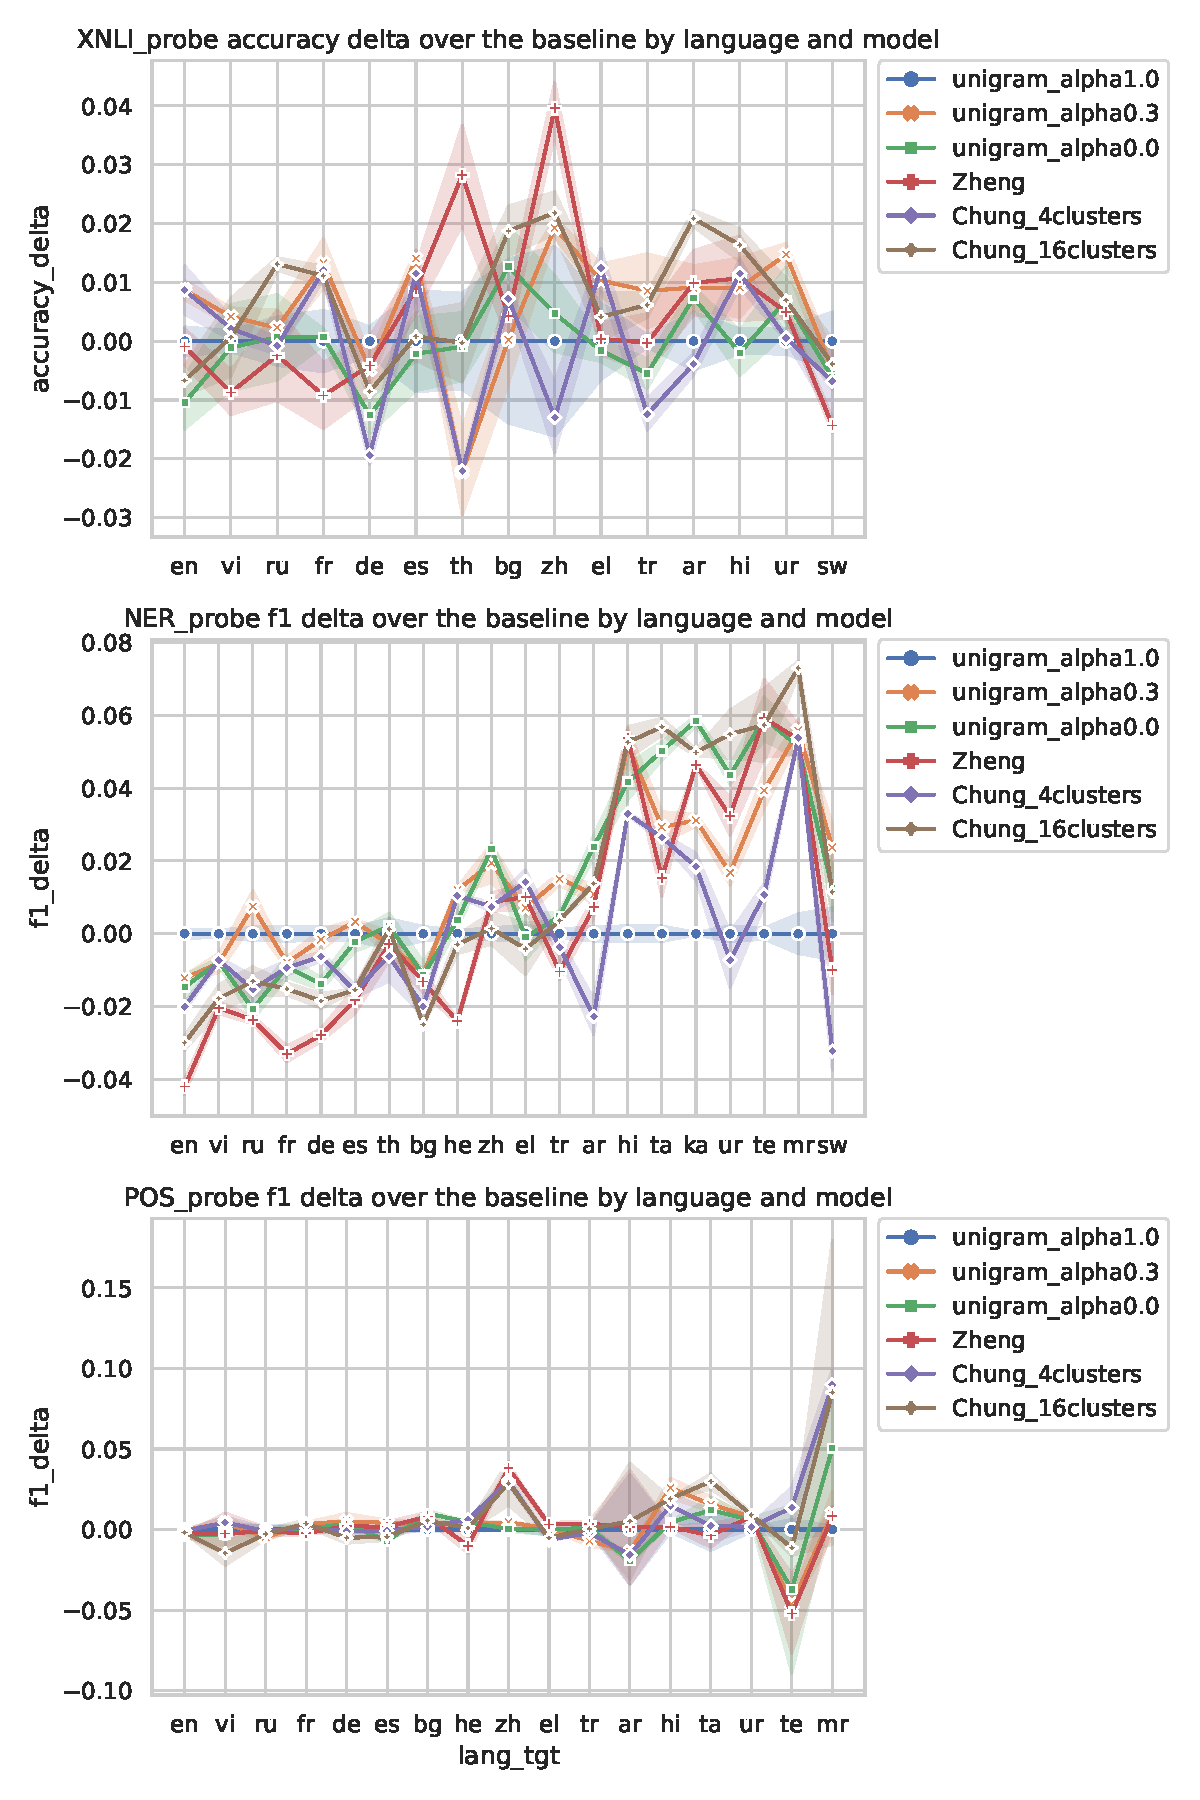
\includegraphics[width=0.8\textwidth]{figures/probe_detailed_inlanguage_over_baseline.pdf}
    \caption{We zoom in on the in-language results from Figure \ref{fig:probe_overall_inlanguage} and compare the performance of the balanced tokenizers against the unbalanced Unigram tokenizer with $\alpha=1.0$ over all tested languages for the tasks. In the case of the word-level tasks, especially in the case of named entity recognition, we observe a clear trend in line with our tokenizer investigations in \ref{fig:chung_vs_alphas}. The balancing methods improve the language representations for word-level tasks. For the sentence-level tasks, we do not observe any systematic effects. This might be in part because the NLI task does not include 4 of our low-resource languages. The error bands are one standard deviation computed from the three probe training runs with different random seeds.}
    \label{fig:probe_overall_inlanguage_over_baseline}
\end{figure}

In \autoref{fig:probe_overall_inlanguage_over_baseline}, we see the in-language results laid out by language. We see a large effect of the probe training language on the NER F1 score and to some degree an effect on the POS F1. We do not see a systematic effect on NLI. For NER, we see the effect of the tokenizer language balance reminiscent of the results in \autoref{fig:zheng_vs_alphas} and \autoref{fig:chung_vs_alphas}. For high-resource languages, we observe a decrease in performance across the board. This is counterbalanced by a larger increase in performance for the low-resource languages. The effect seems to be largest for the $\alpha=0.0$ Unigram tokenizer,ě Zheng method and Chung with 16 clusters. For $\alpha=0.3$ Unigram and Chung with 4 clusters, we see a similar effect but with a smaller magnitude, which is in line with our observations in \autoref{fig:chung_vs_alphas}. In the case of POS, we do see more variance in results towards the low-resource languages but the effect is not as clear as for NER. We see significant improvements with Zheng and Chung methods on Chinese which correspond to the AR improvement for Chinese for the Zheng method in \autoref{fig:zheng_vs_alphas} but we do not see any difference in Chinese tokenizer metrics in the case of Chung (\autoref{fig:chung_vs_alphas}). We also see some improvements in Hindi, Tamil, and Marathi. For Telugu, we see a surprising drop for all methods except Chung with 4 clusters. Note that the variance in the results is larger for the low-resource languages because of smaller test sets.


\begin{figure}[H]
    \centering
    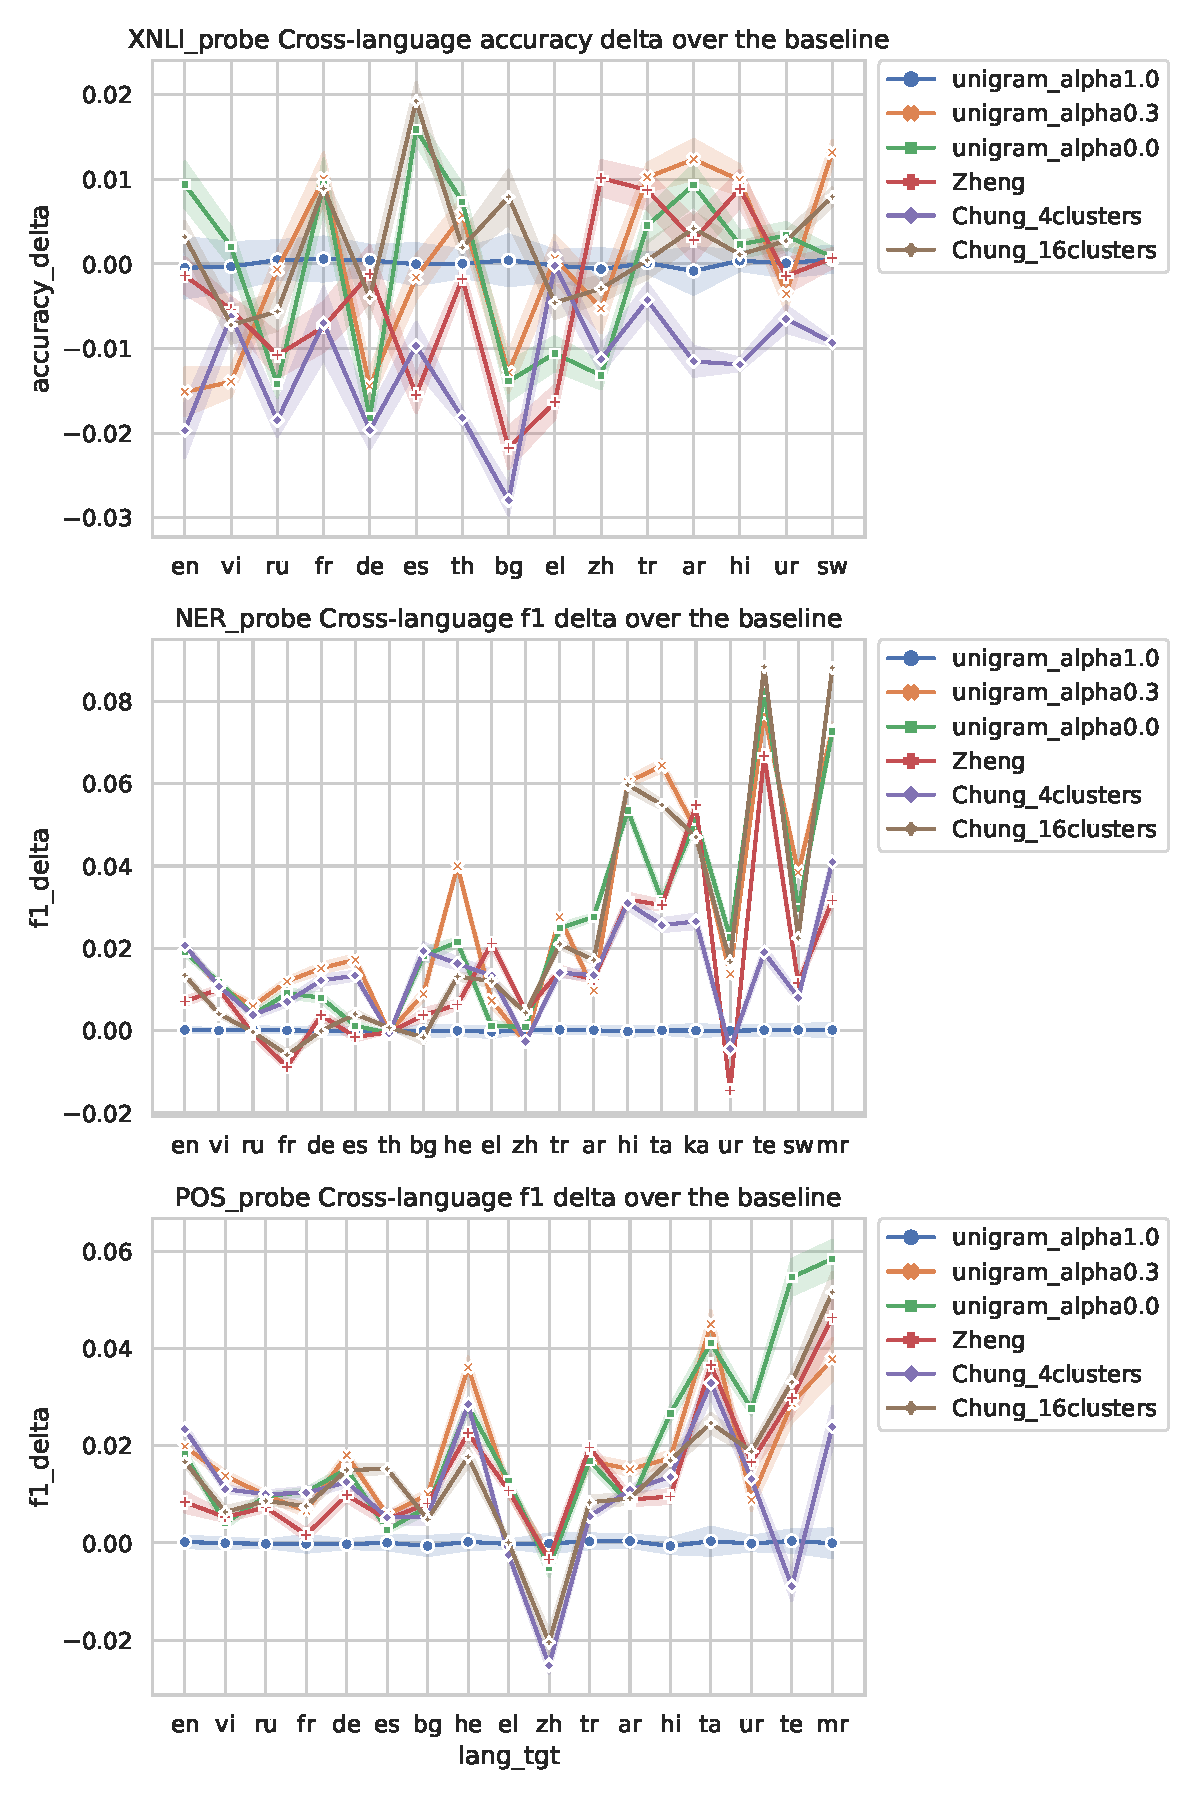
\includegraphics[width=0.8\textwidth]{figures/probe_detailed_crosslanguage_over_baseline_lang_tgt.pdf}
    \caption{Here we investigate in detail the cross-lingual results from Figure \ref{fig:probe_overall_crosslanguage} with comparison to the unbalanced Unigram tokenizer with $\alpha=1.0$. We observe that word-level task transfers behave in line with the tokenizer investigations in \ref{fig:chung_vs_alphas}. Moreover, it seems that both high-resource and low-resource languages benefit from the balancing methods, although the change is most clear on the low-resource side. For the sentence-level tasks, we do not observe any systematic effects. The value for each language and model is computed by averaging the difference in cross-lingual performance for the given \textit{target} language over the baseline. In other words for a given language L we compute the mean performance over all probe trainings done on languages other than L and then evaluate them on language L.}
    \label{fig:probe_overall_crosslanguage_over_baseline}
\end{figure}

We turn our attention to the cross-language results in \autoref{fig:probe_overall_crosslanguage_over_baseline}. Here we again do not see any patterns in the NLI task, other than an overall drop in performance for Chung with 4 clusters, for which we do not have an explanation. On the other hand, we see clear patterns in NER and POS tasks. For both tasks, we see that the performance for low-resource languages is improved over the unbalanced baseline. Moreover, we see that the balancing has a net positive effect even for the high-resource languages, although the effect is not as pronounced as for the low-resource languages. In the NER task, we see that the Chung method with 4 clusters does not seem to improve on low-resource language as much as the other methods. 

Lastly, we plot the differences in tokenizer metrics against the differences in downstream task scores in scatter matrices. In \autoref{fig:probe_overall_inlanguage_scattermatrix} we show the in-language results and in \autoref{fig:probe_overall_crosslanguage_scattermatrix} we show the cross-language results. In the case of in-language results, we see that for the NER and POS tasks, there is a significant Spearman correlation between the differences in tokenizer metrics and the differences in task performance (0.84 and 0.34 Spearman correlation respectively). For the NLI task, we do not observe any significant correlations. This is in line with our observations from the language-level results (\autoref{fig:probe_overall_inlanguage_over_baseline}). In the case of cross-language results, we observe significant, low, negative Spearman correlations between JSD and word-level tasks NER and POS (-0.21 and -0.22 respectively). We also see significant correlations between CPT/AR and all downstream tasks (0.14 for NLI, 0.39 for NER, and 0.29 for POS)\footnote{Because for cross-lingual transfer we test pairs of languages, we compute the combined CPT for the pair of languages as an average between the CPT of the source and target languages.}.

Collecting all our observations together, we see that the tokenizers that aim to balance low-resource and high-resource languages do influence the results of downstream tasks compared to an unbalanced tokenizer. We see that the effect varies by task and language. Generally, we see a high influence on word-level tasks (NER and POS) and no significant influence on NLI. In the case of in-language results, the effect of increasing the vocabulary allocation for low-resource languages and decreasing allocation for high-resource languages is clear for the NER task (\autoref{fig:probe_overall_inlanguage_over_baseline}). In the case of cross-lingual transfer, this effect is clear on both word-level tasks and, interestingly, is a net positive even for the high-resource tasks (\autoref{fig:probe_overall_crosslanguage_over_baseline}). For all cases where the balancing effect is clear (NER in-language, NER/POS cross-language), the best overall performance is achieved by the Unigram tokenizer trained on a balanced train set with $\alpha=0.0\text{ and }0.3$ (\autoref{fig:probe_overall}). For in-language POS, we see the best performance for the Chung method. To quantify the strength of the influence of tokenizer improvement on task improvement, we plot the metrics and downstream results in a scatterplot matrix and compute Spearman correlations between them. For all cases where the balancing effect is clear, we see significant correlations between the differences in tokenizer metrics and the differences in downstream task performance (\autoref{fig:probe_overall_inlanguage_scattermatrix} and \autoref{fig:probe_overall_crosslanguage_scattermatrix}). In general, the correlations we observe suggest that improving vocabulary allocation (CPT, AR) has a positive effect on in-language and cross-language performance on word-level tasks. Moreover, higher vocabulary overlap (lower JSD) also seems to have a positive effect on word-level tasks, although the effect is smaller. 
% Moreover, we also observe significant correlations between inlanguage POS and CPT/AR and significant, low correlation between crosslanguage NLI and CPT/AR

\begin{figure}[H]
    \centering
    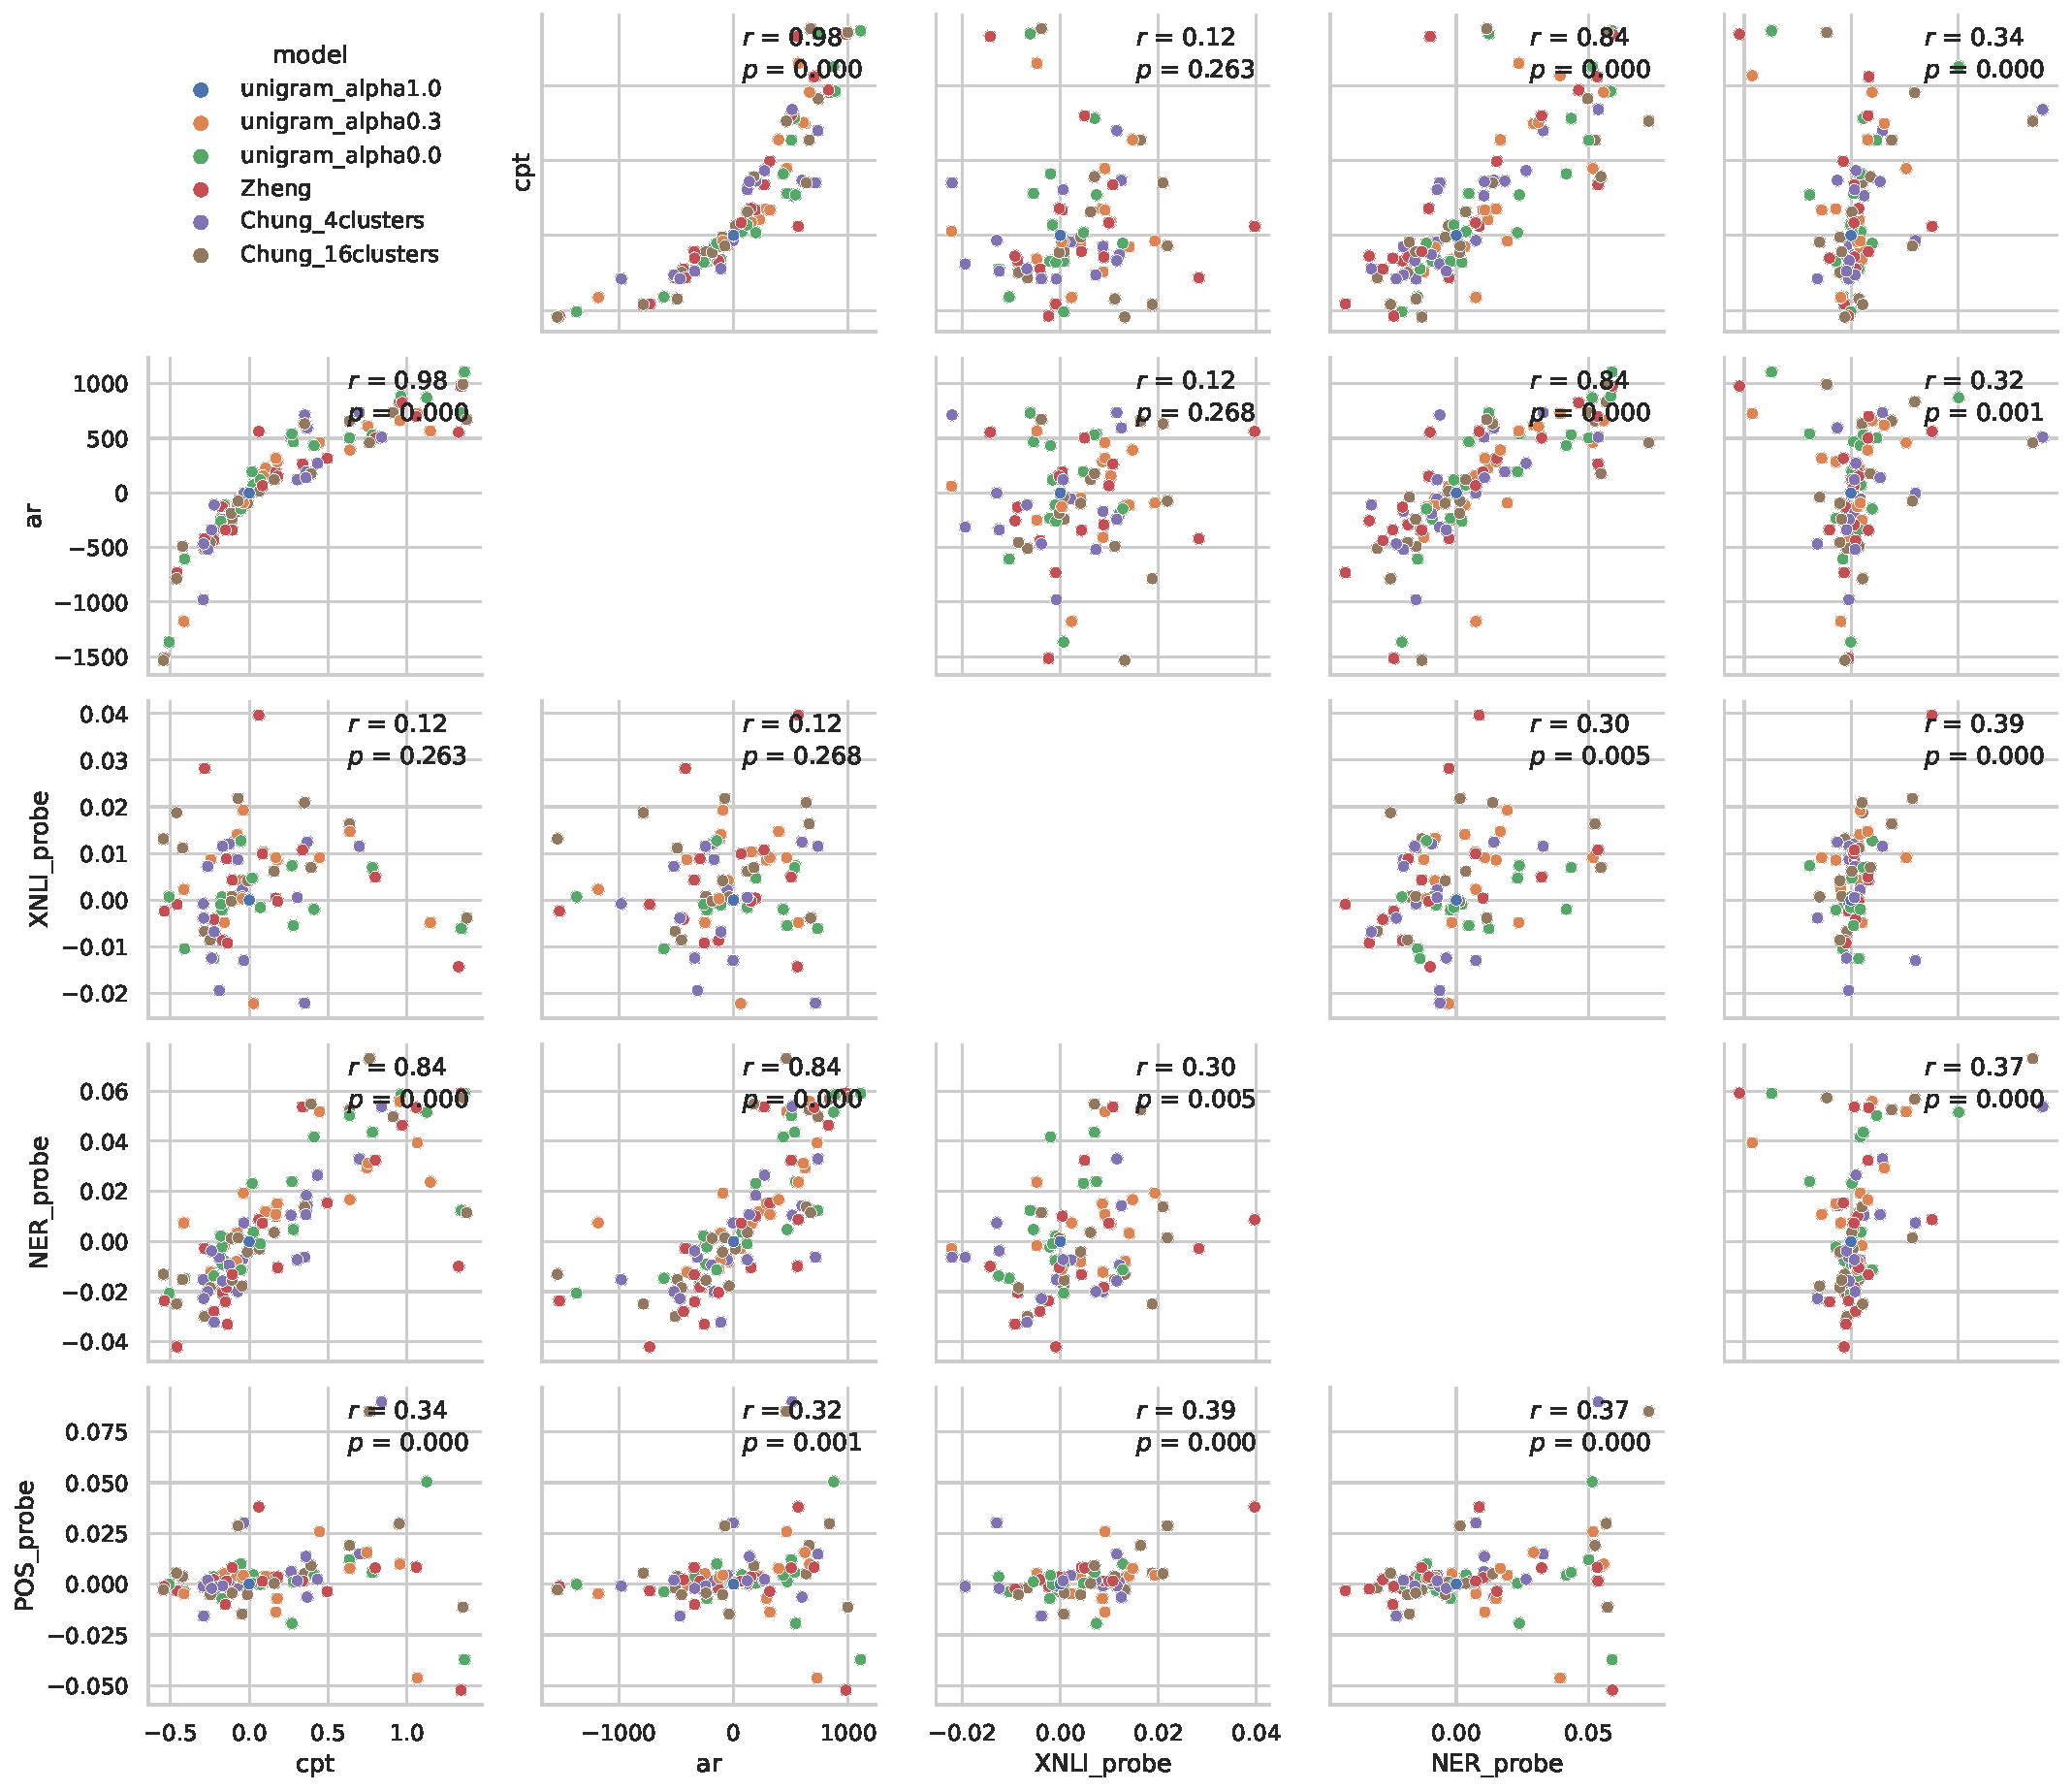
\includegraphics[width=\textwidth]{figures/probe_detailed_inlanguage_scattermatrix.pdf}
    \caption{We visualize the in-language results from Figure \ref{fig:probe_overall_inlanguage} in a scatter matrix. We \tomaszrep{center the results for each language and then plot the differences from the mean performance against the differences in our tokenizer metrics}{substract mean result across three tokenization mwethods from per-language results}. We see significant Spearman correlations for the NER and POS tasks, although for POS the correlation is low. For the NLI task, we do not observe any significant correlations.}
    \label{fig:probe_overall_inlanguage_scattermatrix}
\end{figure}

\begin{figure}[H]
    \centering
    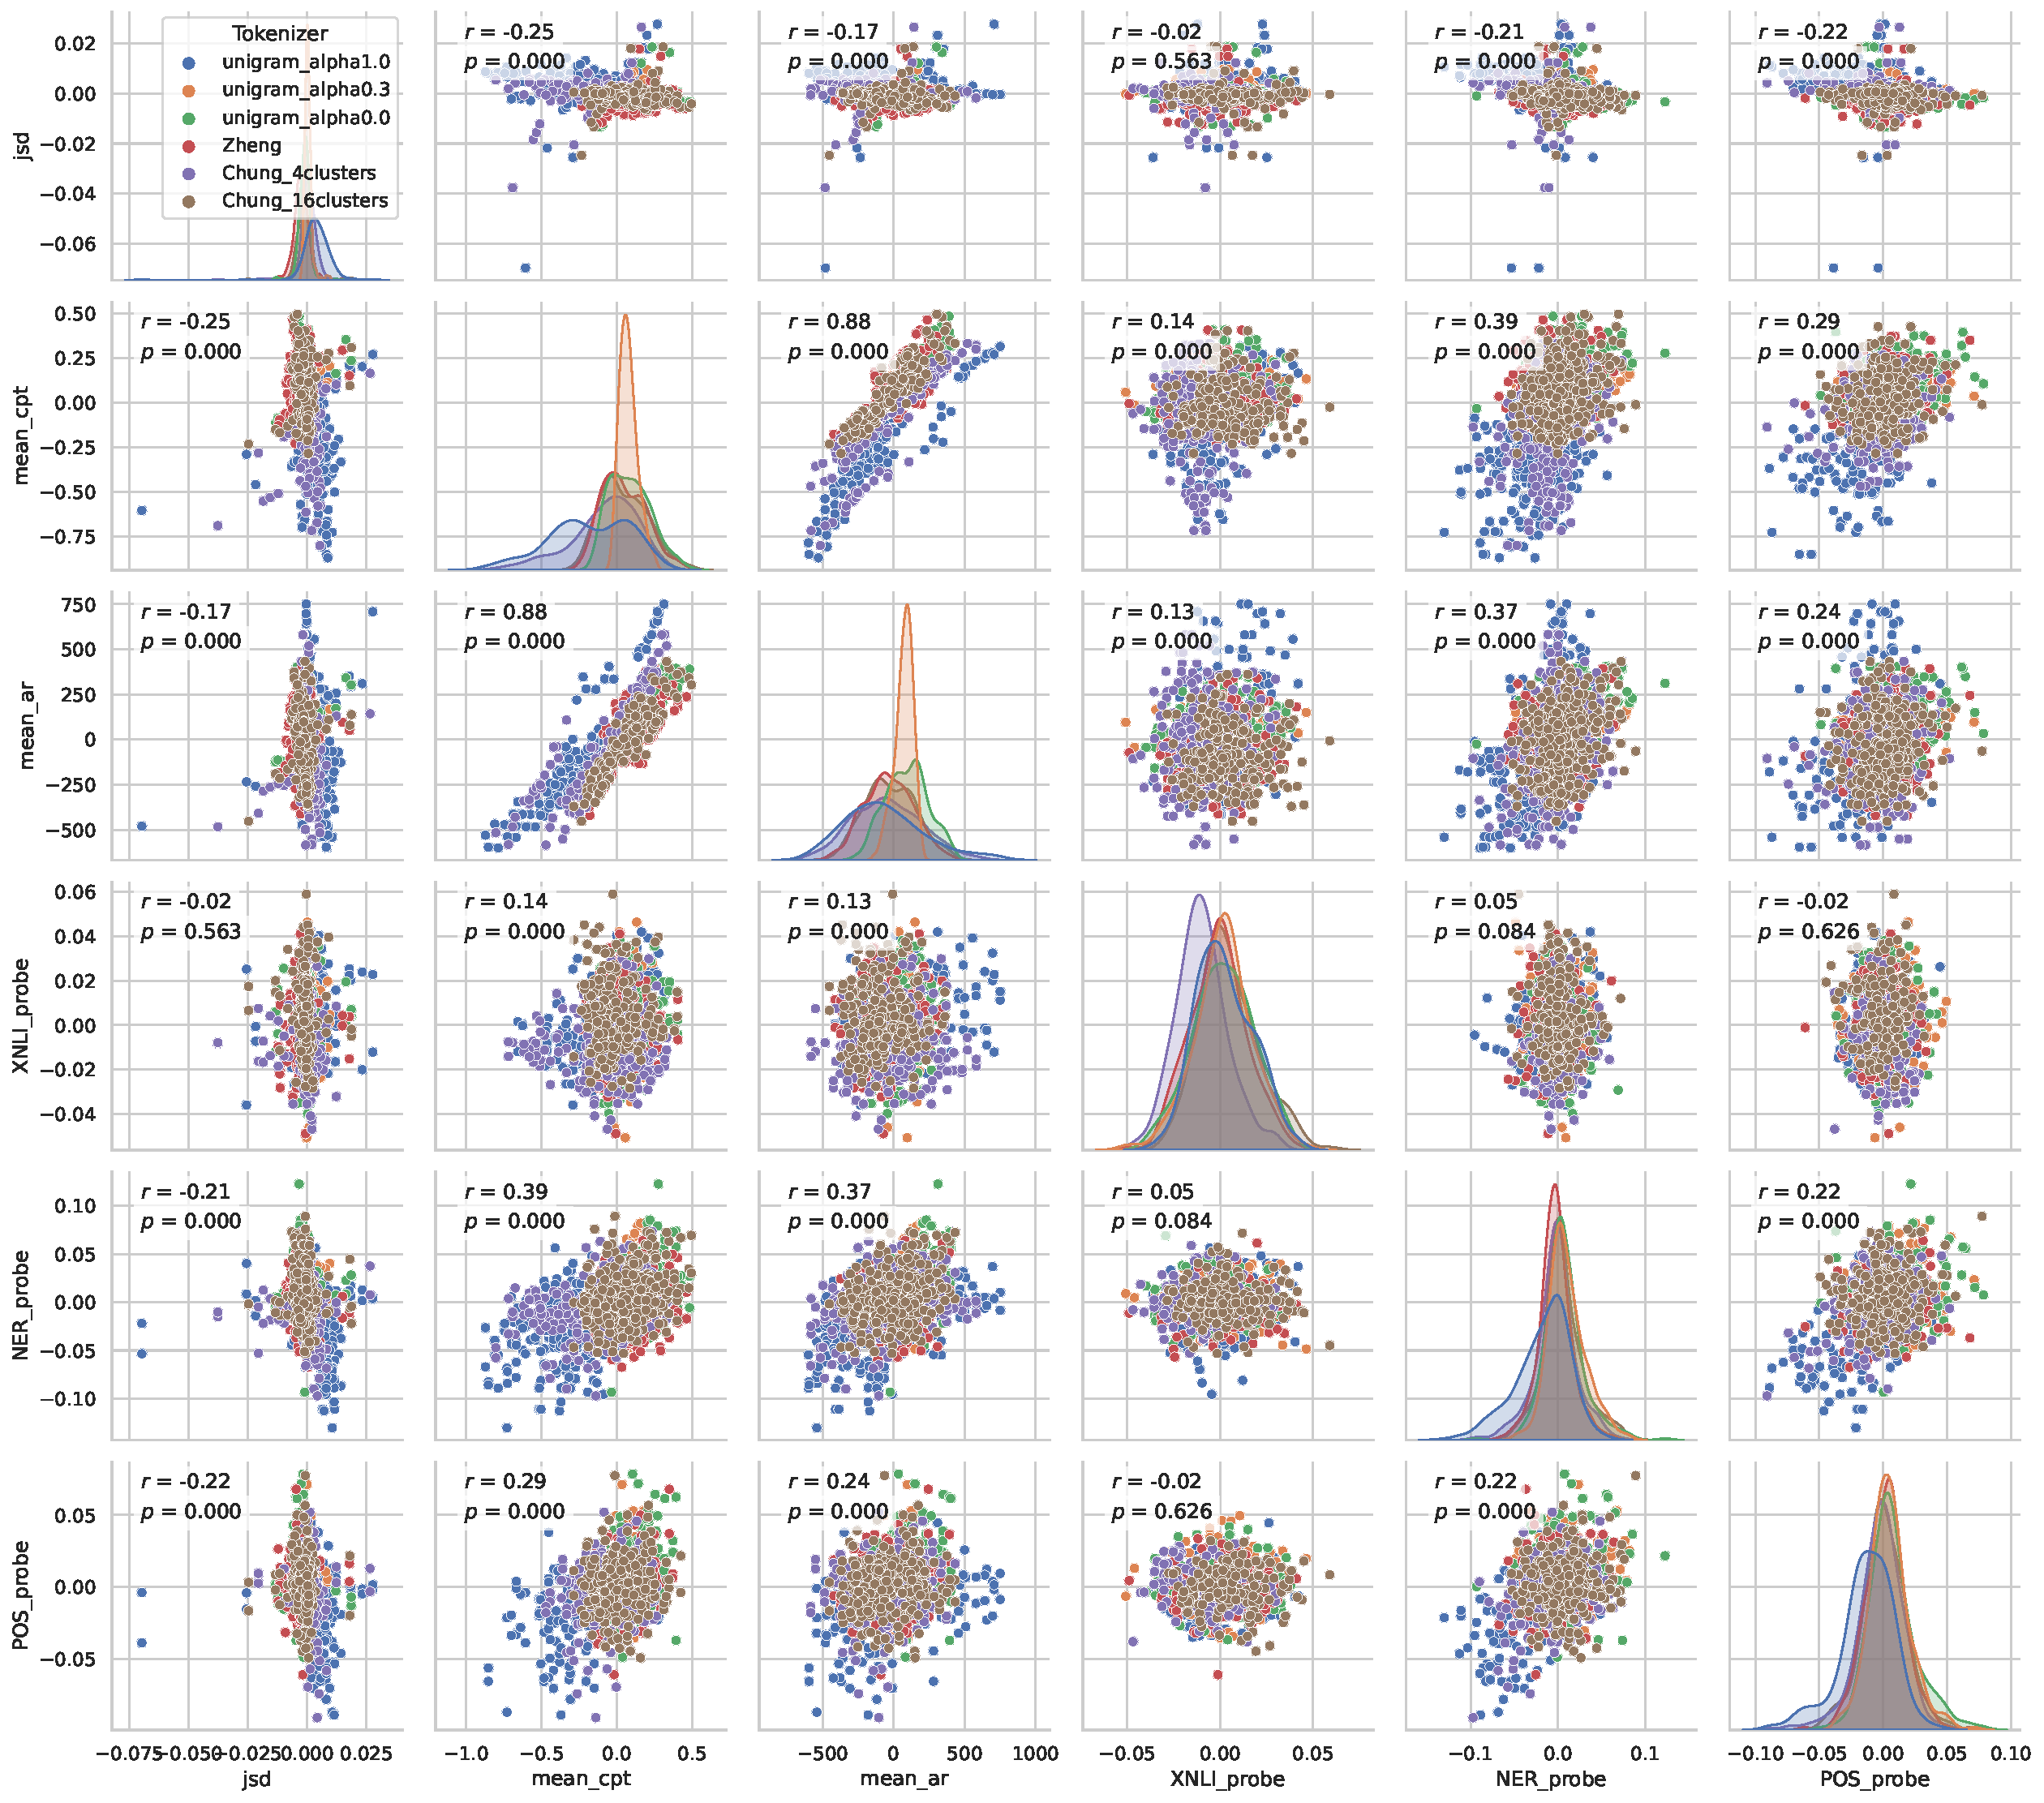
\includegraphics[width=\textwidth]{figures/probe_detailed_crosslanguage_scattermatrix.pdf}
    \caption{We visualize the cross-language results from Figure \ref{fig:probe_overall_crosslanguage} in a scatter matrix. We \tomaszrep{center the results for each language and then plot the differences from the}{substract mean performance across the three models from the language pairs results} of vocabulary overlap metric (JSD) and the combined CPT/AR of the source and target languages. We see significant, very low negative correlations between JSD and F1 scores for the NER and POS tasks and higher, significant correlations between combined CPT and F1 scores. This suggests that the word-level tasks benefit only very slightly from an increase in overlap (decrease in JSD) and an increase in token length in source and target languages. For the NLI task, we observe a significant, low correlation between combined CPT/AR and NLI accuracy. This suggests that the cross-lingual transfer for sentence-level tasks benefits from an increase in token length in source and target languages.}
    \label{fig:probe_overall_crosslanguage_scattermatrix}
\end{figure}

% visualization idea:

% - visualization of tokenizer balance difference is too noisy to see the differences between methods
%     - smoothing num_lines_per_language vs cpt
%     - or fitting a line
%     - something that highlights if one balancing method is better than another

% \section{Preliminary experiments}
% \subsection{The importance of training data size}
% \subsection{Differences in tokenizer implementations}
% \section{Reproduction of baselines}
% \section{Document-level clustering method}
% \section{Extrinsic evaluation}


% - replication of the previous work
%     - Chung
%         - reproductions in Overlap-based Vocabulary Generation Improves Cross-lingual Transfer Among Related Languages

%     - Liang
%         - they use 900k vocab, they compare their model to XLM-R which is not fair!
%             - they discuss it in section 6.4
%         - reproductions: https://github.com/stefan-it/xlm-v-experiments
%             - For XQuAD they did not reproduce the improvements
%             - For MasakhaNER they reproduced the improvements
%             - TODO: could use bootstrapping to show whether the improvements are significant

% replications of Chung, Liang
% https://github.com/stefan-it/xlm-v-experiments

% - our beta experiments point to the randomness of the output - the smooth sweep across the beta values seems to produce quite noisy outpus
